% Definición de la clase del documento
\documentclass[a4paper, 11pt]{book} % A4 paper and 11pt font size

% Entrada y salida de texto
\usepackage[T1]{fontenc}
\usepackage[utf8]{inputenc}
\usepackage[sfdefault]{roboto} % Option 'sfdefault' only if the base font of the document is to be sans serif

% Idioma
\usepackage[spanish, es-tabla]{babel} % Selecciona el español y el uso de la palabra "tabla" en lugar de "cuadro"

% Información reutilizable
\newcommand{\asunto}{Trabajo de Fin de Grado}
\newcommand{\titulo}{SmartU}
\newcommand{\tituloEng}{SmartU}
\newcommand{\subtitulo}{Desarrollo de un espacio colaborativo de ideas y proyectos}
\newcommand{\subtituloEng}{Development of a coworking space for ideas and projects}
\newcommand{\grado}{Grado en Ingeniería Informática}
\newcommand{\autor}{Juan José Jiménez García}
\newcommand{\email}{juanjojg@correo.ugr.es}
\newcommand{\tutor}{Miguel Gea Megías}
\newcommand{\escuela}{Escuela Técnica Superior de Ingenierías Informática y de Telecomunicación}
\newcommand{\departamento}{Departamento de Lenguajes y Sistemas Informáticos}
\newcommand{\universidad}{Universidad de Granada}
\newcommand{\ciudad}{Granada}
\providecommand{\keywords}{COMPLETAR ESTO}
\providecommand{\keywordsEng}{COMPLETE THIS}

% Otros paquetes importantes para el proyecto
\usepackage{url}
\usepackage{graphicx}
\usepackage{fancyhdr}
\usepackage{pdfpages}
\usepackage[hidelinks]{hyperref}

% Información del archivo
\hypersetup{
  pdfauthor = {\autor\ (\email)},
  pdftitle = {\titulo: \subtitulo},
  pdfsubject = {\asunto},
  pdfkeywords = {\keywords},
  pdfcreator = {LaTeX, con la distribución TeX Live},
  pdfproducer = {pdflatex}
}

% Modificación para que las páginas en blanco no tengan cabecera
\makeatletter
\def\clearpage{
  \ifvmode
    \ifnum \@dbltopnum =\m@ne
      \ifdim \pagetotal <\topskip
        \hbox{}
      \fi
    \fi
  \fi
  \newpage
  \thispagestyle{empty}
  \write\m@ne{}
  \vbox{}
  \penalty -\@Mi
}
\makeatother

% Definición del estilo de las cabeceras
\pagestyle{fancy}
\fancyhf{}
\fancyhead[LO]{\leftmark}
\fancyhead[RE]{\rightmark}
\fancyhead[RO,LE]{\textbf{\thepage}}
\setlength{\headheight}{1.5\headheight}

% Redefinición de comandos
\renewcommand{\chaptermark}[1]{\markboth{\textbf{#1}}{}}
\renewcommand{\sectionmark}[1]{\markright{\textbf{\thesection. #1}}{}}
% \renewcommand{\lstlistingname}{Fragmento de código}
% \renewcommand{\lstlistlistingname}{Índice de fragmentos de código}

% Creación de comandos
% \newcommand{\HRule}{\rule{\linewidth}{0.5mm}}
% \newcommand{\bigrule}{\titlerule[0.5mm]}

% Ajuste para minimizar el fragmentado de listados
% \lstnewenvironment{listing}[1][]
%   {\lstset{#1}\pagebreak[0]}{\pagebreak[0]}


\begin{document}

\begin{titlepage}

\newlength{\centeroffset}
\setlength{\centeroffset}{-0.5\oddsidemargin}
\addtolength{\centeroffset}{0.5\evensidemargin}

\noindent\hspace*{\centeroffset}

\begin{minipage}{\textwidth}

\centering


\includegraphics[width=0.9\textwidth]{logo_ugr}\\[1.4cm]

\textsc{\Large\asunto\\[0.2cm]}
\textsc{\grado}\\[1cm]

{\Huge\bfseries\titulo\\}
\noindent\rule[-1ex]{\textwidth}{3pt}\\[3.5ex]
{\large\bfseries\subtitulo}

\end{minipage}

\vspace{1.5cm}
\noindent\hspace*{\centeroffset}

\begin{minipage}{\textwidth}

\centering

\textbf{Autor}\\{\autor}\\[2.5ex]
\textbf{Tutor}\\{\tutor}\\[1.5cm]


\includegraphics[width=0.3\textwidth]{logo_etsiit}\\[0.1cm]

\textsc{\escuela}\\
\textsc{---}\\
\ciudad, \today\\

\end{minipage}

\end{titlepage}

\frontmatter
\cleardoublepage
\thispagestyle{empty}

\begin{center}
{\LARGE\bfseries\titulo: \subtitulo}\\
\end{center}
\begin{center}
\autor
\end{center}

\bigskip
\noindent{\textbf{Palabras clave}: \textit{\keywords}\\

\section*{Resumen}
Este documento detalla mi trabajo y participación en el proyecto multidisciplinar llevado a cabo en la Universidad de Granada.\\

\textbf{SmartU} nace del trabajo en equipo realizado por un grupo de estudiantes y sus tutores, como respuesta a un problema habitual de la vida universitaria, que es el fomento de proyectos de carácter multidisciplinar.\\

Lo que se pretende con este trabajo es crear una plataforma basada en un formato de \textbf{red social} que permita a los estudiantes publicar proyectos e ideas y con ello encontrar a otros estudiantes de diversas disciplinas que quieran unirse para llevar a cabo la idea.\\

SmartU pretende ser un apoyo y una forma de fomentar más el \textbf{trabajo en equipo}, algo que la sociedad actual demanda mucho en sus puestos de trabajo y que no termina de fraguar del todo en las universidades. \\

Como resultado de este trabajo, también se obtienen una serie de \textbf{resultados y conclusiones} sobre cómo ha sido este primer ``proceso piloto'' de equipo multidisciplinar, que servirá de ayuda para mejorar en el futuro los problemas encontrados.

\cleardoublepage
\thispagestyle{empty}

\begin{center}
{\LARGE\bfseries\tituloEng: \subtituloEng}\\
\end{center}
\begin{center}
\autor
\end{center}

\bigskip
\noindent{\textbf{Keywords}: \textit{\keywordsEng}\\

\section*{Abstract}
This final degree document explains my work and collaboration on the multidisciplinary project made on the University of Granada.\\

\textbf{SmartU} is the result of the teamwork carried out by a group of students and their tutors in response to a common problem in the university life, which is the promotion of multidisciplinary projects.\\

This work aims to create a \textbf{social network based} web platform which allows students to publish projects and ideas in order to find another students from other specialties who want to join to carry it out.\\

SmartU is meant to be a support to promote \textbf{work in team}, since it's something highly required by today's jobs but it's not very popular in universities.\\

As a result from this project, we also got a bunch of \textbf{results and conclusions} about how well this first multidisciplinary project was, which will be used to improve in the future the found problems.

\chapter*{}
\thispagestyle{empty}

\noindent\rule[-1ex]{\textwidth}{2pt}\\[4.5ex]

Yo, \textbf{\autor}, alumno de la titulación \textbf{\grado} de la \textbf{\escuela} de la \textbf{\universidad}, con DNI 76655977J, autorizo la ubicación de la siguiente copia de mi Trabajo de Fin de Grado en la biblioteca del centro para que pueda ser consultada por las personas que lo deseen.

\vspace{6cm}

\noindent \textbf{Fdo: \autor}

\vspace{2cm}

\begin{flushright}
\ciudad, a \today
\end{flushright}

\chapter*{}
\thispagestyle{empty}

\noindent\rule[-1ex]{\textwidth}{2pt}\\[4.5ex]

D. \textbf{\tutor}, profesor del \textbf{\departamento} de la \textbf{\universidad}.

\vspace{0.5cm}

\textbf{Informa:}

\vspace{0.5cm}

Que el presente trabajo, titulado \textit{\textbf{\titulo: \subtitulo}}, ha sido realizado bajo su supervisión por \textbf{\autor}, y autoriza la defensa de dicho trabajo ante el tribunal que corresponda.

\vspace{0.5cm}

Y para que conste, expide y firma el presente informe en \ciudad, a \today.

\vspace{1cm}

\textbf{El tutor:}

\vspace{5cm}

% \begin{figure}[H]
% \includegraphics[width=0.3\textwidth]{firma_tutor}
% \end{figure}

\noindent\textbf{\tutor}

\chapter*{Agradecimientos}
\thispagestyle{empty}

\vspace{1cm}

Quisiera agradecer a mi familia todo el apoyo que me han brindado no solo durante mi etapa en la universidad, sino también en el colegio y el instituto. Gracias por toda vuestra ayuda y cariño. \\

Gracias a mis amigos y amigas de la ETSIIT de Granada, los mejores compañeros de trabajo que he conocido y con quienes he pasado momentos geniales. \\

A mis profesores, tanto a los buenos como a los ``no tan buenos'', les agradezco que me hayan ayudado a ser quien soy hoy con su atención y esfuerzo por querer transmitir sus valiosos conocimientos. \\

Y a mis compañeros del TFG, con quienes he compartido estos últimos meses dando forma a este proyecto, muchas gracias. Especialmente a Emilio, y a mi tutor Miguel.


\begingroup
\let\cleardoublepage\clearpage
  \tableofcontents
%  \listoffigures
%  \listoftables
%  \lstlistoflistings
\endgroup

\newpage
\thispagestyle{empty}

\mainmatter
\chapter{Introducción}

Prueba de capítulo.

% \chapter{Objetivos}
\label{ch:objetivos}

Este capítulo recoge los objetivos iniciales marcados para este proyecto, una vez descrita la situación inicial en la que nos encontramos tras la lectura del primer capítulo. Recapitulando lo visto anteriormente, podemos describir el proyecto de la siguiente forma:\\

\textit{``\textbf{SmartU} es un proyecto multidisciplinar en el que se va a llevar a cabo una experiencia piloto de un equipo de trabajo formado por estudiantes y profesores de diferentes áreas del conocimiento, encontrar la forma de fomentar este tipo de proyectos que son poco habituales, y además, servir como base para encontrar una metodología de trabajo que funcione y sea perfeccionada con el paso del tiempo.''}\\

El proyecto de SmartU (nombre procedente de la combinación de los términos \textit{\textbf{Smart}} y \textit{\textbf{University}}) se ideó originalmente como un proceso piloto en el que, al mismo tiempo que se trabaja en \textit{elaborar} algo, que en este caso es la metodología de trabajo multidisciplinar, nos servía también como prueba de concepto de lo que estábamos investigando, ya que el equipo es precisamente multidisciplinar.\\

Vamos a esquematizar los objetivos de este trabajo en diferentes puntos:

\begin{itemize}
    \item \textbf{Gestión y coordinación del equipo:} Como forma de promover este tipo de equipos, el propio desarrollo se realizará sobre un equipo multidisciplinar, para analizar su progreso y detectar ventajas y fallos que deberían de subsanarse con el tiempo.
    \item \textbf{Creación de una metodología de trabajo multidisciplinar:} A lo largo del proyecto, se recopilará la información sobre cómo se ha trabajado, para así crear una especie de \textit{``Manual de trabajo de equipos multidisciplinares''}.
    \item \textbf{Creación de las plataformas software:} En el primer año de funcionamiento del proyecto, se quiere crear las primeras versiones de las plataformas web y móvil de creación y difusión de proyectos, como forma de demostrar el concepto sobre el que estamos trabajando y para comenzar a atraer la atención del público objetivo.
    \item \textbf{Marketing del proyecto:} Es importante crear una campaña de publicidad y difusión del proyecto que permita que la gente conozca lo que estamos haciendo, mostrando las ventajas que aportaría a la sociedad en general y el enriquecimiento que supondría para la docencia universitaria.
\end{itemize}

Estos son los pilares básicos del proyecto. En sucesivas iteraciones del proyecto, pueden salir más, pero estos son los que inicialmente consideramos más importantes y como manera de empezar a dar forma al mismo.\\

Quiero destacar dos de los puntos mencionados anteriormente, ya que son en los que me he centrado yo principalmente y desarrollaré con más detalle a lo largo de esta memoria:

\begin{itemize}
    \item \textbf{Gestión y coordinación del equipo.}
    \item \textbf{Creación de plataforma software.}
\end{itemize}

\subsection{Gestión y coordinación del equipo}
Uno de mis propósitos en este proyecto es actuar de coordinador del mismo, gestionar los recursos y documentos que se generen a lo largo del tiempo y organizar y dirigir las reuniones que se lleven a cabo. Esto se desarrolla con más atención en el \textit{capítulo \ref{ch:metodologia}}.

\subsection{Creación de plataforma software}
Se pretenden desarrollar dos apliaciones de gestión de proyectos de carácter multidisciplinar. Una de ellas es la aplicación móvil de SmartU, cuyo desarrollo queda a cargo de mi compañero Emilio. El otro es el de la aplicación web, del cual me encargo yo.\\

Dada la naturaleza incipiente del proyecto, y el hecho de que también cuento con la responsabilidad de gestión del mismo, no se esperaba desde el principio que se llegase a completar al 100\% el desarrollo de dicha aplicación web, pero dado que este proyecto es software libre, se da la oportunidad de que en el futuro, el código sea mejorado y ampliado con más funcionalidades.\\

Aun con ello, se definieron unos aspectos importantes que desde el principio iba a cumplir la aplicación web:

\begin{itemize}
    \item La interfaz de usuario debe ser clara e intuitiva.
    \item La interfaz de usuario debe ser adaptable a todo tipo de tamaños de pantalla.
    \item La interfaz de usuario ha de ser lo menos intrusiva posible y dejar espacio a los contenidos relevantes.
    \item El código ha de ser claro y estar documentado de forma correcta para que otras personas puedan continuar y mejorar la aplicación.
\end{itemize}

\section{Estado del arte}
\subsection{Proyectos similares}
Como parte de la investigación realizada sobre este proyecto, encontramos algunas plataformas con una idea subyacente similar a la que estamos trabajando: prima la colaboración en equipo, el acercamiento de sectores de la sociedad y la creación de proyectos.

\begin{itemize}
    \item \textbf{Medialab UGR} \cite{medialabugr} se concibe como un espacio de encuentro para el análisis, investigación y difusión de las posibilidades que las tecnologías digitales generan en la cultura y en la sociedad en general.
    \item \textbf{Link by UMA-ATech} \cite{linkuma} reúne a asociaciones, estudiantes, empresas, emprendedores y todo tipo de expertos para compartir ideas, aprender y crecer juntos. En definitiva, Link es un espacio para crear grandes proyectos (imagen \ref{linkumaimage}).
    \item \textbf{LinkedIn} \cite{linkedin} es una comunidad social orientada a las empresas, a los negocios y el empleo. Partiendo del perfil de cada usuario, que libremente revela su experiencia laboral y sus destrezas en un verdadero currículum laboral, la web pone en contacto a millones de empresas y empleados.
    \item \textbf{Kickstarter} \cite{kickstarter} es un sitio web de micromecenazgo en el que los usuarios pueden publicar sus proyectos y obtener financiación de la gente para poder llevarlo a cabo. En caso de que el proyecto haya tenido éxito financiándose, los donantes reciben recompensas relacionadas con el proyecto que se va a realizar.
\end{itemize}

\begin{figure}
    \centering
    
\includegraphics[scale=0.7]{linkuma}
    \caption{Evento de \textit{Yes We Tech} en Link - \textcopyright\ Geek and Tech Girls \cite{linkimage}}}
    \label{linkumaimage}
\end{figure}

\subsection{Usabilidad y UX}
En el campo de la usabilidad y la \textit{User Experience} (UX) se ha dicho mucho con el objetivo de encontrar la clave de un sistema que sea usable y amigable para todos los grupos de usuarios de tecnología que existen actualmente. Se hace necesario para lograr éxito que las interfaces sean sencillas de entender y claras, con una estructura que no haga que el usuario desinstale la aplicación o cierre la pestaña del navegador.\\

Por ello, para este proyecto, en lo que corresponde al trabajo de desarrollo web, he decidido construir mi aplicación web en base a unos principios de diseño actuales y que siguen creciendo con el paso del tiempo.

\subsubsection{Diseño adaptable o \textit{responsive}}
El diseño adaptable establece que un sistema informático (ya sea una página web, un programa de ordenador o una aplicación móvil) debe ser \textbf{reactivo} a la interacción del usuario con el mismo y al entorno en el que se encuentra. Esto quiere decir que ha de ``adaptarse'' a todo tipo de dispositivos donde se esté ejecutando o visualizando. \cite{responsivelink}\\

Ya sea en una pantalla de 24 pulgadas, o un smartphone de 5, el sistema ha de ser capaz de mostrar la misma información y de proporcionar la misma funcionalidad, \textbf{reorganizando los contenidos} de la interfaz para que nada quede inaccesible. En la figura \ref{water} podemos ver de forma gráfica el concepto que aquí se expone.\\

En este sentido, existe un framework de diseño adaptable que nos facilita la tarea de crear un sistema usable en todo tipo de formatos de pantalla, \textbf{Bootstrap} \cite{bootstrap}. Proporciona un conjunto de elementos para el \textit{``layout''} de la aplicación y objetos de interacción como pestañas, botones, paneles, etc.

\begin{figure}
    \centering
    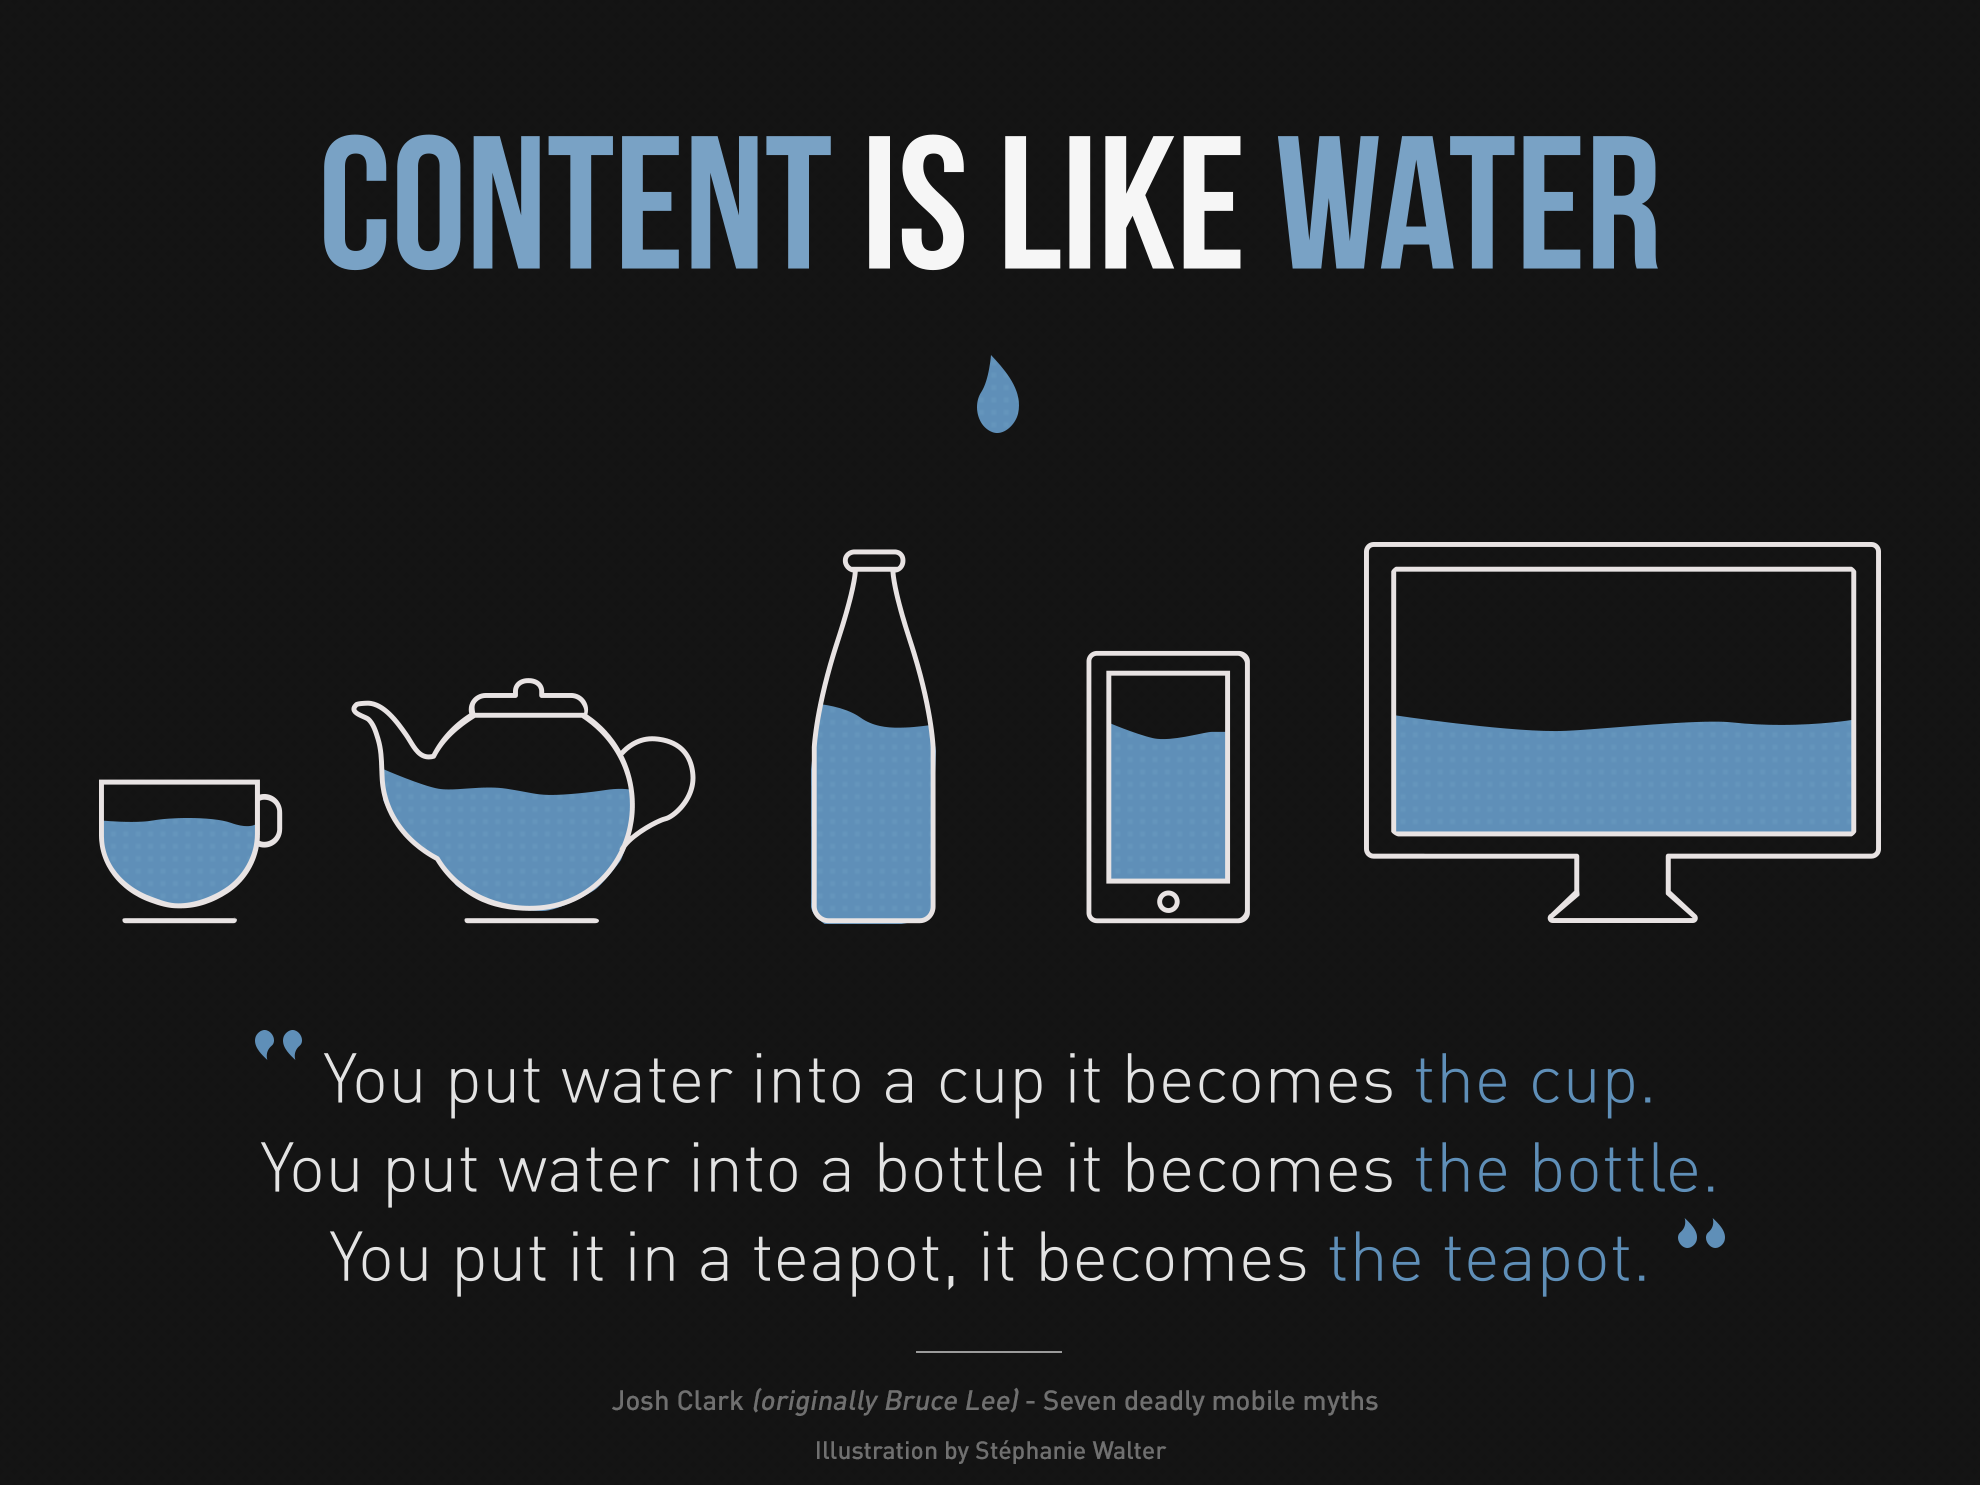
\includegraphics[scale=0.165]{water}
    \caption{\textit{``El contenido es como el agua''} - \textcopyright\ Clark y Walter \cite{contentwater}}
    \label{water}
\end{figure}

% \chapter{Metodología de trabajo multidisciplinar}
\label{ch:metodologia}

Este capítulo describe la metodología de trabajo que se ha seguido para llevar a cabo el proyecto. Detalla las tareas y actividades que se planean realizar, así como el conjunto de herramientas de trabajo que se han visto con mayor utilidad para lograr un flujo de trabajo más productivo.\\

Como se mencionó anteriormente, mi tarea consistirá no solo en el desarrollo de una plataforma web, sino también la gestión del equipo, a modo de \textit{project manager}. Como tal, nos encontramos ante la situación de organizar a un equipo de personas que mayormente no son del mismo grado, por lo que pueden no estar acostumbrados o ser conocedores de las mismas herramientas que utlizamos habitualmente.\\

En el presente capítulo se tratará de buscar aquellas herramientas que sean sencillas y tengan una curva de aprendizaje baja. El motivo es múltiple, ya que se han de encontrar recursos aptos para todos, que no los abrumen o les frustren, para que así los utilicen y beneficie al proyecto en si.

\section{Líneas de trabajo}
En el nacimiento de este equipo, se planteó que debemos funcionar de forma similar a una Startup \cite{startup}. Siguiendo esa lógica, trabajamos sobre una idea innovadora para resolver un problema complejo, empleando la tecnología para llegar a cumplir el objetivo.\\

Sobre el concepto de SmartU, nacen una serie de \textbf{líneas de trabajo} que son importantes para lograr un producto completo y útil para su público objetivo, por ello es necesario que se trabaje en ellas de forma correcta.

\begin{description}
    \item[Software] La línea de trabajo donde crear aplicaciones web y móviles que el público objetivo usará con el fin de facilitar la tarea de la creación de proyectos multidisciplinares.
    \item[Marketing] Esta línea de trabajo concentra sus esfuerzos en la búsqueda de formas de promoción adecuadas al público y que garanticen que SmartU llegue al máximo número de personas posibles. Destacamos por ejemplo el uso de las redes institucionales ya existentes para dar difusión, así como la creación de redes sociales propias de la plataforma como forma de acercamiento a los demás.
    \item[Diseño gráfico] La identidad visual es el reto al que se enfrenta esta línea de trabajo. Se ha de encontrar un estilo y diseño diferenciador que además sea agradable al usuario, y que de alguna forma represente los conceptos sobre los que trabajamos, como por ejemplo el concepto principal de ciudades inteligentes.
    \item[Plan de empresa] El plan de empresa tiene como objetivo encontrar una estrategia de negocio que sirva para que esta \textit{startup} sea viable en el futuro.
\end{description}

\section{El equipo}
El equipo de trabajo se ha compuesto de diferentes \textbf{profesores y estudiantes} de diversas disciplinas de la universidad. Podemos ver su nombre y ocupación en la \textbf{tabla \ref{miembrossmartu}}. Todos han aportado conocimientos de su campo al proyecto para intentar lograr los mejores resultados, recibiendo opiniones y puntos de vista muy diferentes que ayudan y complementan.

\begin{table}
    \begin{center}
        \begin{tabular}{|p{4.5cm}|p{6.5cm}|}
            \hline
                \rowcolor{Gray}\multicolumn{1}{|c|}{\textbf{Integrante}}
                & \multicolumn{1}{|c|}{\textbf{Ocupación}} \\
            \hline
                Juan Árbol Gutiérrez & Estudiante de CC.EE. y Empresariales \\
            \hline
                Irene Castillo Pardo & Estudiante de Comunicación y Audiovisuales \\
            \hline
                Emilio Chica Jiménez & Estudiante de Ingeniería Informática \\
            \hline
                Victoria Guerra Molina & Estudiante de Comunicación y Audiovisuales \\
            \hline
                Juan José Jiménez García & Estudiante de Ingeniería Informática \\
            \hline
                Javier Labrat Rodríguez & Estudiante de Ingeniería Informática \\
            \hline
                Germán Zayas Cabrera & Estudiante de Bellas Artes \\
            \hline
                Miguel Gea Megías & Profesor de Ingeniería Informática \\
            \hline
                Guillermo Maraver Tarifa & Profesor de CC.EE. y Empresariales \\
            \hline
                Alejandro Grindlay Moreno & Profesor de Ingeniería Civil \\
            \hline
        \end{tabular}
        \caption{Integrantes del proyecto multidisciplinar SmartU}
        \label{miembrossmartu}
    \end{center}
\end{table}

\subsection{Obligaciones del equipo}
A cada uno de los miembros del equipo se le asigna un rol o tarea. Es importante que cada uno se dedique a algo relacionado con sus conocimientos, de esta manera se esperaba conseguir mejores resultados, al \textbf{delegar en la persona adecuada la tarea adecuada}. Podemos ver el reparto de roles en la \textbf{tabla \ref{rolessmartu}}.\\

\begin{table}
    \begin{center}
        \begin{tabular}{|p{5cm}|p{6cm}|}
            \hline
                \rowcolor{Gray}\multicolumn{1}{|c|}{\textbf{Integrante/s}}
                & \multicolumn{1}{|c|}{\textbf{Rol o tarea}} \\
            \hline
                Juan Árbol Gutiérrez & Emprendedor y gestor de estrategia empresarial \\
            \hline
                Juan José Jiménez García & Gestor de proyecto y desarrollador de software \\
            \hline
                Emilio Chica Jiménez & Gestor tecnológico y desarrollador de software \\
            \hline
                Irene Castillo Pardo y Victoria Guerra Molina & Gestoras de audiovisuales \\
            \hline
                Germán Zayas Cabrera & Diseñador gráfico \\
            \hline
                Javier Labrat Rodríguez, Miguel Gea Megías, Guillermo Maraver Tarifa y Alejandro Grindlay Moreno & Tutores y consultores para dudas \\
            \hline
        \end{tabular}

        \caption{Roles y tareas de los miembros del equipo SmartU}
        \label{rolessmartu}
    \end{center}
\end{table}

En la \textbf{tabla \ref{tareassmartu}} se puede ver un resumen general del trabajo que va a realizar cada uno de los miembros del equipo.

\newpage
\begin{longtable}{|m{4.5cm}|m{6.5cm}|}
    \hline
        \rowcolor{Gray}\multicolumn{1}{|c|}{\textbf{Integrante}}
        & \multicolumn{1}{|c|}{\textbf{Aportaciones}} \\
    \hline
        Juan Árbol Gutiérrez & \begin{itemize}
            \item Organizador del Design Thinking y Brainstorming
            \item Creador del plan estratégico de empresa
            \item Responsable de realización de entrevistas a posibles usuarios objetivo del sistema
            \item Presentador del proyecto en la Facultad de Ciencias de la Actividad Física y del Deporte
        \end{itemize} \\
    \hline
        Irene Castillo Pardo & \begin{itemize}
            \item Colaborador en el Design Thinking y Brainstorming
            \item Creadora del video de presentación del proyecto
            \item Creación del making of del proyecto
        \end{itemize} \\
    \hline
        Emilio Chica Jiménez & \begin{itemize}
            \item Creador de la aplicación móvil del proyecto
            \item Organizador del Design Thinking y Brainstorming
            \item Moderador de seminario de tecnologías emergentes
            \item Gestor de reuniones
        \end{itemize} \\
    \hline
        Victoria Guerra Molina & \begin{itemize}
            \item Colaborador en el Design Thinking y Brainstorming
            \item Investigadora de una campaña de difusión del proyecto en redes sociales y medios de publicidad
        \end{itemize} \\
    \hline
        Juan José Jiménez García & \begin{itemize}
            \item Organizador del Design Thinking y Brainstorming
            \item Gestor del proyecto
            \item Creador de la aplicación web
            \item Coordinador y documentador de reuniones
            \item Coordinador del repositorio de archivos y calendario
        \end{itemize} \\
    \hline
        Javier Labrat Rodríguez & \begin{itemize}
            \item Presentador del proyecto en la Facultad de Ciencias de la Actividad Física y del Deporte
            \item Creador de un proyecto que servirá de muestra para nuestro sistema SmartU
        \end{itemize} \\
    \hline
        Germán Zayas Cabrera & \begin{itemize}
            \item Colaborador en el Design Thinking y Brainstorming
            \item Creador de la identidad visual del proyecto
            \item Creador del diseño de la página web de presentación del proyecto
        \end{itemize} \\
    \hline
        Miguel Gea Megías & \begin{itemize}
            \item Creador de la idea original
            \item Agrupador de los miembros del equipo
            \item Consejero para el desarrollo del proyecto
            \item Colaborador en el Design Thinking y Brainstorming
            \item Gestor de las reuniones
        \end{itemize} \\
    \hline
        Guillermo Maraver Tarifa & \begin{itemize}
            \item Colaborador en el Design Thinking y Brainstorming
            \item Consejero de Juan para el desarrollo del proyecto
            \item Consejero de marketing y promoción del proyecto
        \end{itemize} \\
    \hline
        Alejandro Grindlay Moreno & \begin{itemize}
            \item Colaborador en el Design Thinking y Brainstorming
            \item Consejero para el desarrollo del proyecto
        \end{itemize} \\
    \hline
    \caption{Aportaciones de los miembros del equipo}
    \label{tareassmartu}
\end{longtable}

\subsection{Dependencias entre miembros del equipo}
En un proyecto multidisciplinar, es muy importante \textbf{encontrar sinergias} entre los miembros del mismo, es decir, encontrar puntos comunes que permitan una colaboración fructuosa entre dos personas. Así, el trabajo que teníamos que hacer cada uno se vería más reforzado al contar con el punto de vista y la ayuda proporcionada por otra persona de diferente disciplina.\\\\

Las sinergias son muy populares en el mundo empresarial, en concreto entre los campos de \textit{marketing} o economía, y se valora mucho el resultado obtenido de esa cooperación. Por ello, en este tipo de proyectos, es muy deseable realizar un esfuerzo por encontrarlas.

\section{Gestión del trabajo}
Como gestor del proyecto (una de mis obligaciones además del desarrollo de software), junto con mi tutor Miguel realizaremos la \textbf{organización del trabajo} con el objetivo de conseguir la mayor agilidad posible para la comunicación y para documentar los progresos. En las siguientes secciones de este apartado se describe con más detalle lo que se va a realizar para cada uno de los puntos de gestión.

\subsection{Temporización}
Uno de los aspectos más importante a la hora de gestionar un proyecto es la temporización, es decir, definir los tiempos que se estima requerirán las posibles tareas que surjan para llevarlo a cabo. Es vital tener en mente siempre que los cambios existen y con una alta probabilidad van a aparecer, por lo que se ha de estar preparado para asumirlos e intentar integrarlos en el proyecto, intentando que afecte lo menos posible a la planificación inicial.\\

Para este apartado se puede hacer uso del \textbf{diagrama de Gantt}, que establece tareas y el tiempo requerido de estas, así como los recursos necesarios (tanto humanos como materiales) para poder realizarlas. Permite estudiar mejor posibles bloqueos y dependencias entre tareas, y ver de forma más gráfica si el tiempo se está distribuyendo bien entre integrantes y en el espacio.

\subsection{Comunicación}
Un proyecto de esta índole necesita de varias \textbf{reuniones}, donde poder debatir asuntos y tomar decisiones, así como para realizar ciertas técnicas creativas de generación de ideas y establecer las funcionalidades de los productos a desarrollar. Estos puntos son tratados más adelante en esta documentación.\\

Es deseable que las reuniones sean siempre, en la medida de lo posible, en el mismo lugar, como forma de hacer más estable el proceso del proyecto y no crear demasiada confusión al equipo. De no poder hacer esto posible, se puede intentar hacer uso de instalaciones de la universidad como salas insonorizadas o aulas de seminario, pensadas para trabajos en equipo. Contar con proyector o pizarra en la sala es muy recomendable para hacer una mejor dinámica de reuniones.\\

Debido a la diferencia de disciplinas que presentaban los integrantes, se hace necesario establecer un \textbf{horario semanal} donde se ajuste la disponibilidad de todos los miembros para que puedan asistir el máximo número de personas. Este horario no ha de ser fijo obligatoriamente, semana a semana se puede actualizar para un mejor ajuste a las circunstancias que puedan tener los miembros del equipo.\\

Podemos describir el \textbf{proceso de organización de reuniones} de la siguiente manera:

\begin{enumerate}
    \item Como gestión previa a una reunión, se ha de hacer lo siguiente:
    \begin{enumerate}
        \item Se \textbf{comunica a los gestores} la necesidad de realizar una reunión para tratar un asunto importante del proyecto.
        \item Los gestores se \textbf{reunen} para establecer los puntos de la próxima reunión.
        \item Se \textbf{comunica al resto del equipo} la necesidad de realizar la reunión y se les pide que indiquen en el horario los días que mejor le convenían, para encontrar el punto común para que puedan asistir todos.
        \item Los profesores, debido a la posibilidad que presentan de \textbf{reservar salas de reuniones} más adecuadas que los que los estudiantes tenían permitido, se pueden encargar de encontrar sitio para celebrar la reunión en base a la disponibilidad de los asistentes.\\
        También se pueden encargar de comprobar que la sala que se reserve cuente con material adecuado para la reunión, como un \textbf{proyector, pizarra}, etc.
        \item Se establece en el calendario oficial del proyecto (con \textbf{Google Calendar} \cite{googlecalendar}) y se informaba al resto del equipo por el medio correspondiente.
    \end{enumerate}
    \item Al comenzar la reunión, se han de resumir los puntos tratados en la \textbf{reunión anterior}, a modo de recordatorio y para aquellos miembros que no hubieran podido asistir a dicha reunión. Tras el resumen, se procede a informar de los puntos a debatir en la reunión actual.
    \item Al acabar la reunión se han de comentar los \textbf{nuevos puntos a tratar} de cara a la próxima reunión, y se anotan para no olvidarlos y que los gestores puedan prepararlos.
    \item El gestor del proyecto crea un \textbf{acta de reunión} donde se detallan los puntos debatidos y se apuntan los temas a tratar para la próxima reunión.
\end{enumerate}

Entre las muchas herramientas de comunicación disponibles actualmente, existen algunas muy enfocadas al ámbito profesional, que pueden ser igual de útiles para un entorno de trabajo en equipo universitario. El \textbf{correo electrónico} es un clásico que aun perdura y muchos utilizan, además de aplicaciones de mensajería instantánea como \textbf{WhatsApp}, o el chat de equipos \textbf{Slack}.\\

Se destaca en este punto Slack, al ser una plataforma de comunicación muy pensada para equipos de trabajo de empresas, permitiendo definir canales de comunicación para tratar asuntos concretos, y que agrupen a un subconjunto de personas del equipo, de modo que puedan tratar algo sin molestar al resto de integrantes. Podemos ver una captura de ejemplo de Slack en la imagen \ref{slackimage}.

\begin{figure}
    \centering
    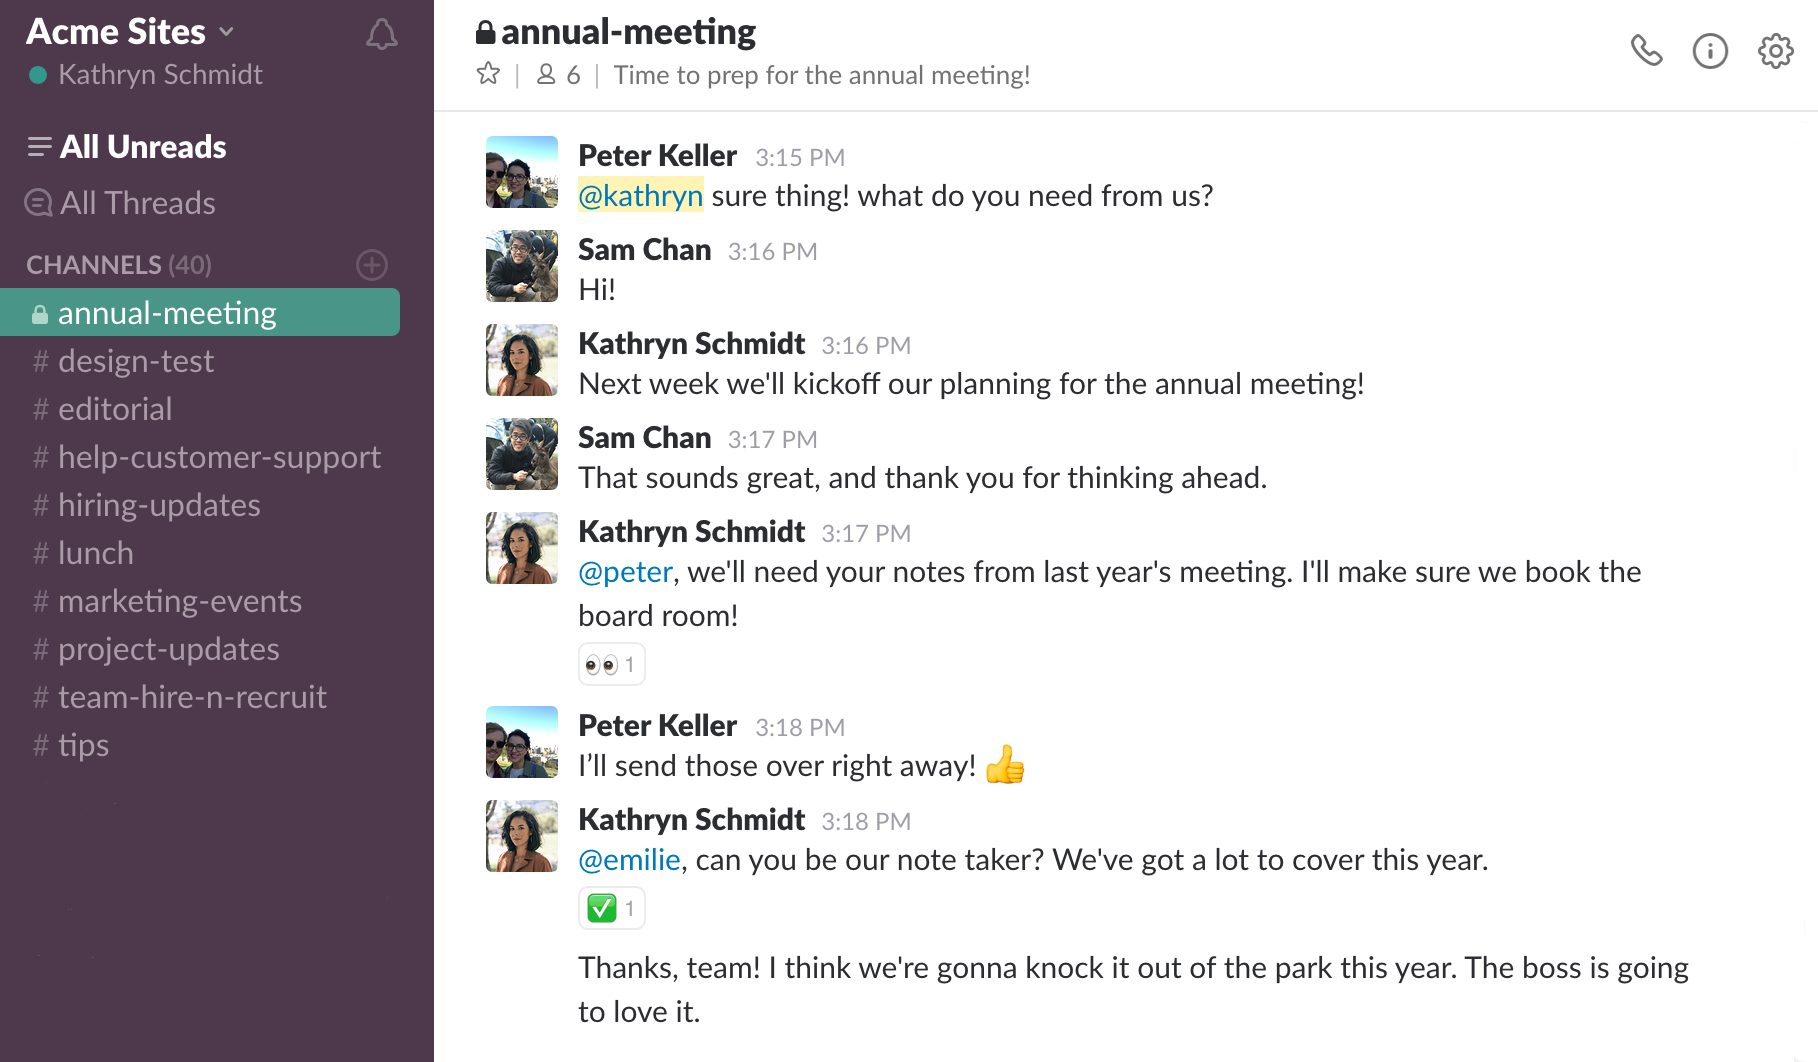
\includegraphics[scale=0.2]{slack}
    \caption{Pantalla principal de Slack - \textcopyright\ Slack}
    \label{slackimage}
\end{figure}

\subsection{Documentación}
Para gestionar la documentación y todo el contenido que el equipo produzca a lo largo del tiempo, es necesario contar con un espacio común de alojamiento de archivos. Para esto se puede optar por utilizar el servicio de almacenamiento en la nube \textbf{Google Drive} \cite{googledrive}.\\

Todos han de tener acceso a dicho directorio online, y ahí se han de ir dejando los documentos que el equipo genere, como pueden ser:
\begin{itemize}
    \item Presentaciones para exponer en reuniones.
    \item Actas de reuniones.
    \item Bocetos de diseño de aplicaciones o de identidad visual.
    \item Calendario semanal actualizado.
\end{itemize}

\subsection{Seminarios y divulgación}
Otro aspecto importante a la hora de realizar un proyecto de este tipo son los seminarios. Los seminarios permiten realizar una presentación y explicación de algún tema o concepto concreto de cualquier área del conocimiento, y generalmente pueden ser para un público más conocedor del tema, o hacerlo más divulgativo para que puedan comprender sus contenidos personas de todos los ámbitos.\\

En un equipo formado por diferentes estudiantes y profesores, es importante dar a conocer conceptos o técnicas habituales en algunas ramas del conocimiento, con el fin de que todos conozcan, no en un nivel avanzado, aspectos importantes para el proyecto, y que a algunos miembros no les resulte extraño o desconocido lo que hacen.\\

Por medio de los seminarios, podemos explicar algo a todo el equipo, y existen diversas técnicas de creatividad que los pueden hacer partícipes en los seminarios, para así motivarlos más y que logren afianzar mejor los nuevos conocimientos.

\subsubsection{Catálogo de seminarios}
Existen multitud de métodos de generación de ideas, que abarcan procesos de análisis, investigación/descubrimiento y definición de estrategias:

\begin{itemize}
    \item Card sorting
    \item Design Thinking
    \item Brainstorming
    \item SCAMPER
    \item Business Model Canvas
\end{itemize}

En esta documentación no vamos a hablar de cada uno de esos métodos, sino que nos centraremos en el que consideramos más interesante y que usaremos en este proyecto, el \textbf{Design Thinking}

\subsubsection{Design Thinking}
Una de las técnicas de creatividad más útiles es la del \textit{Design Thinking}. Tal y como podemos ver en \cite{designthinkinglink}, podemos definirlo como:\\

\textit{``Es un método para generar ideas innovadoras que centra su eficacia en entender y dar solución a las necesidades reales de los usuarios. Proviene de la forma en la que trabajan los diseñadores de producto. De ahí su nombre, que en español se traduce de forma literal como "Pensamiento de Diseño", aunque nosotros preferimos hacerlo como "La forma en la que piensan los diseñadores".''}\\

El Design Thinking es una herramienta muy visual que le da importancia a la experimentación y el prototipado. Su eficacia radica en la capacidad de entender y dar solución a las necesidades reales de los usuarios.\\

Es una técnica muy recomendable y que cada vez se usa más, por lo que es muy recomendable ponerla en práctica con el equipo, ya que puede ser un gran estímulo para obtener ideas, además de que ayuda a que el equipo se conozca mejor y haya más complicidad entre integrantes.

\section{Conclusión}
En este capítulo se han descrito las técnicas y actividades que se pueden realizar para gestionar un equipo multidisciplinar. Los resultados obtenidos tras su aplicación pueden verse en el capítulo \ref{ch:conclusiones}, así como un análisis de los mismos.

% \input{chapters/04_Resultados}
% \chapter{Conclusiones y mejoras para el futuro}

% \chapter{Anexos}
\label{ch:anexos}

\section{Ideas recopiladas de la sesión de \textit{Design Thinking}}
\label{sec:designthinking}
\begin{itemize}
    \item \textbf{Aspectos positivos}
    \begin{itemize}
        \item Pensar y actuar, comprometerme.
        \item ¡Armarse de valor! Empezar y luego ir mejorando aspectos, uno por uno.
        \item Sienten que la universidad no fomenta el trabajo en equipo cuando es algo que las empresas demandan (se ve como algo positivo a aprovechar).
        \item Oigo que las empresas siempre están buscando talentos y gente con ideas para ayudarles a llevarlas a cabo.
        \item Puede dar difusión a una buena idea.
        \item El TFG de mi carrera es muy aburrido (visto como oportunidad).
        \item Veo posibilidades de mejorar la realidad física a través de la realidad virtual. Pensar.
        \item Es una oportunidad de crear proyectos interesantes y experiencias.
        \item Proponer herramientas online y virtuales y generar documentación.
        \item Múltiples posibilidades. Inquietud.
        \item Trabajar duro para llegar a la cohesión. Investigar acerca de todo, el máximo posible. Afrontar el proyecto sin temor al fracaso.
        \item Frustración por no desarrollar una idea propia.
        \item Apostar por ideas innovadoras de TFG. Buscar ideas/productos interesantes para motivar.
        \item Veo un gran distanciamiento entre los distintos campus y no saben lo que pasa entre unos y otros.
    \end{itemize}
    \item \textbf{Ideas}
    \begin{itemize}
        \item Identidad visual.
        \item Comunicación.
        \item Plataforma web.
        \item Jornadas de estudiantes como forma de conocer sus necesidades e incertidumbres.
        \item Fomentar espacios virtuales para comunicación, reuniones y conocimiento.
        \item Fomentar espacios físicos de debate y trabajo (ámbito lúdico, forma de llegar a la sociedad).
    \end{itemize}
    \item \textbf{Objetivos}
    \begin{itemize}
        \item Mapa geográfico de proyectos que permitan acceder al proyecto.
        \item Proyectos conectados entre sí, por tipo.
        \item Hay que crear grupos muy comprometidos y concienciados.
        \item Dificultades, reuniones
        \item Posibilidad de llegar a todos.
        \item Exposición en público.
        \item Crear congresos y seminarios sobre el proyecto interdisciplinar.
        \item Síntesis de ideas para transformarlas en contenido a exponer en redes y otros medios y así dar repercusión al proyecto.
    \end{itemize}
    \item \textbf{Limitaciones}
    \begin{itemize}
        \item No se conoce. Dudas acerca de la viabilidad. No lo entienden. Les atrae como para crear una empresa.
        \item Cómo dar más difusión a los trabajos TFG.
        \item Huimos del tema por miedo a suspender. Vamos a lo fácil para sacar la carrera y no nos complicamos.
        \item Oigo que la gente tiene buenas ideas que le gustaría desarrollar, pero les falta gente que sepa de ciertas cosas.
        \item Cuesta trabajo encontrar tiempo para dedicárselo.
        \item No hay espacios para trabajar en grupo. No hay espacio ni tiempo suficiente para trabajar.
        \item Es un mayor esfuerzo de lo que parece habitual.
        \item No hay tiempo y faltan espacios.
        \item Grandes ideas, propuestas interesantes. Pero hay limitaciones de tiempo y material.
        \item Inseguridad. Ilusión por realizar algo innovador. Falta de un anteproyecto que una las diferentes ramas.
        \item Hay que conformarse con el TFG establecido.
        \item Oigo a la gente quejarse de que trabajar en equipo a veces no sale bien.
        \item No hay tiempo para reuniones y organizar.
        \item Exceso de trámites para realizar un TFG.
        \item Piensan que trabajar en equipo es un engorro y que siempre sale mal.
        \item No existen herramientas para hacer diferentes TFG.
        \item Falta de ayuda por parte de la universidad y el ayuntamiento.
        \item Como ven que es difícil trabajar en equipo, lo que hacen es conformarse con un proyecto más simple que les gusta menos.
        \item Con desesperación, con esperanza, con oportunidades.
        \item Necesidad de implicación (nosotros mismos, menos integrantes). Necesidad de sintetizar las ideas. Si una persona no conoce el proyecto, o quiere participar, una idea clara.
        \item Plazos y forma de organización a veces muy rígida.
        \item Veo que la gente no está motivada a trabajar en equipo y prefieren trabajar solos.
        \item Incertidumbre, amparo, curiosidad.
        \item Inestabilidad, falta de conexión.
    \end{itemize}
\end{itemize}

\section{Actas de reunión del equipo}
\label{sec:actas}
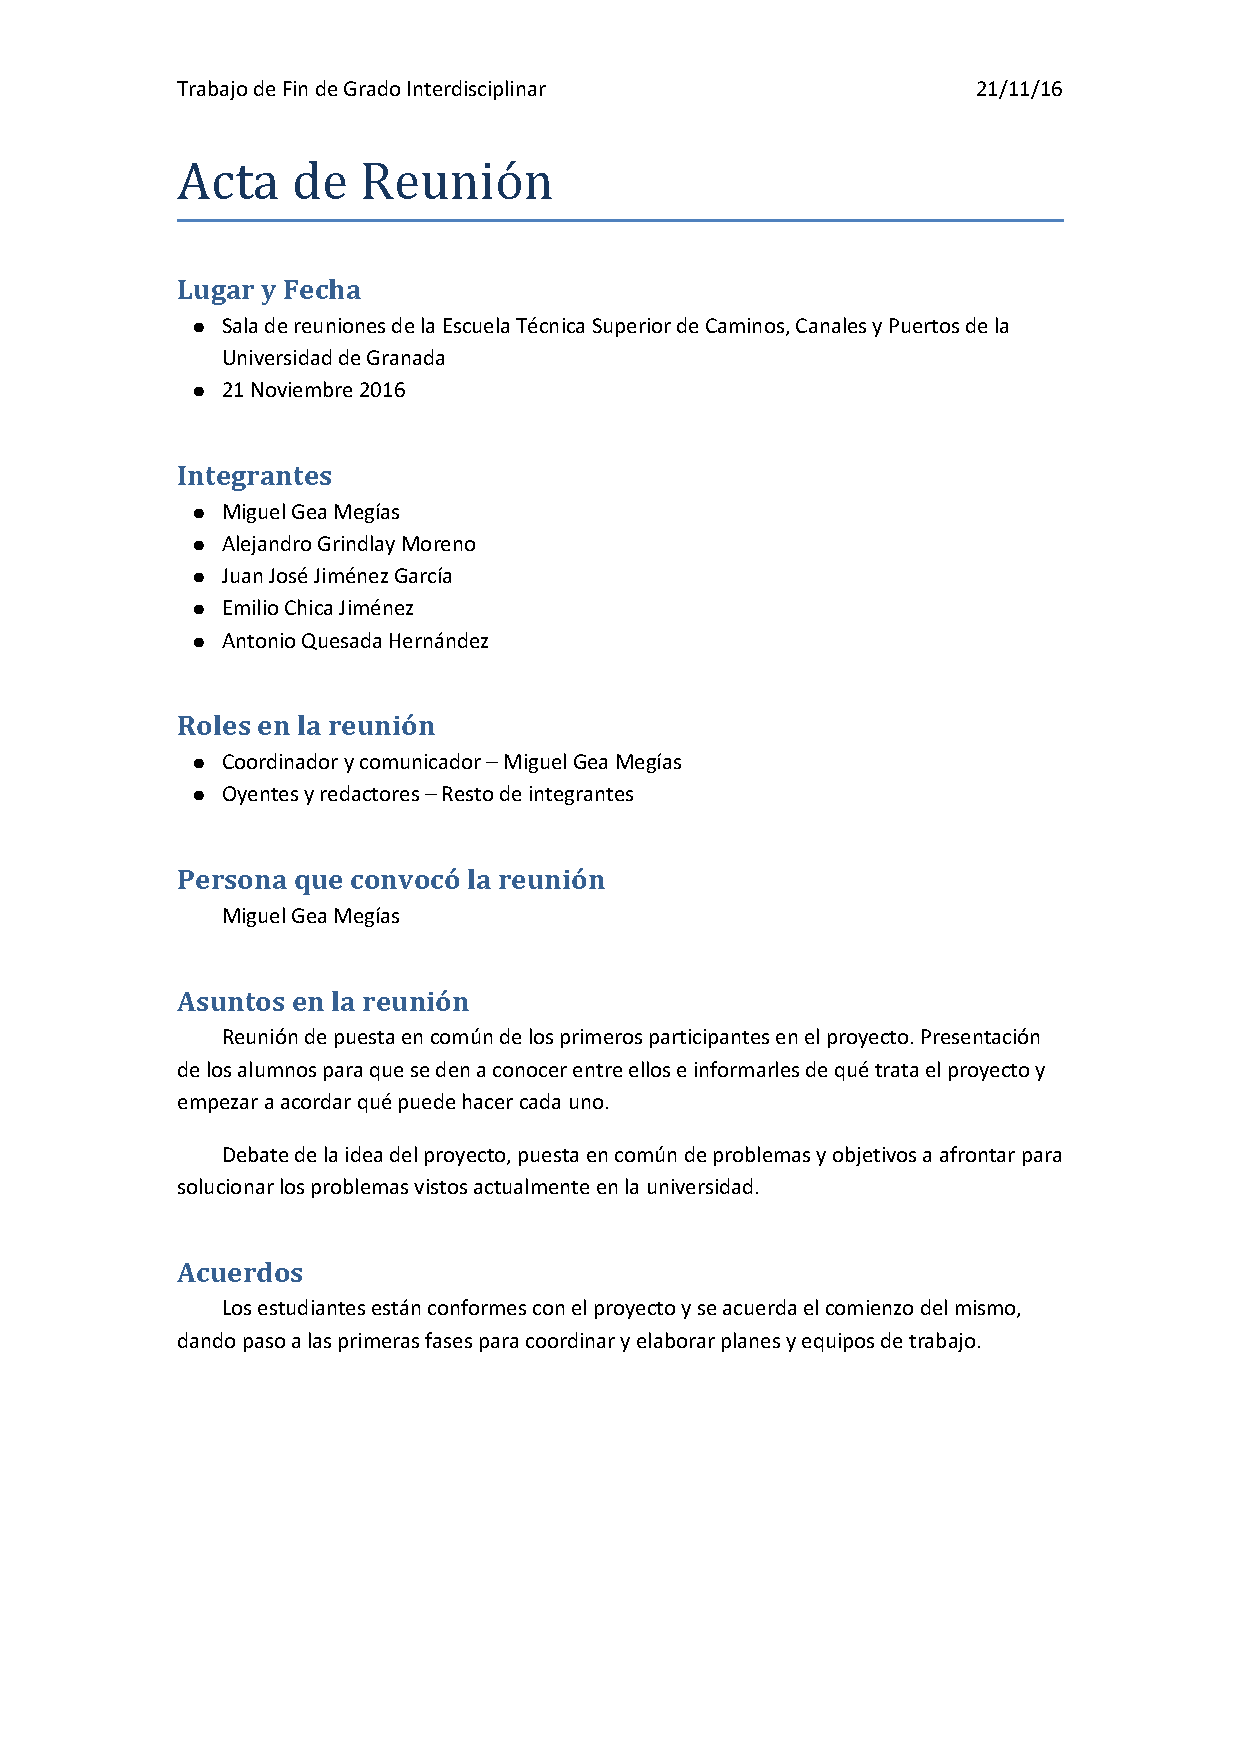
\includepdf[pages=1-]{meetings/01.pdf}
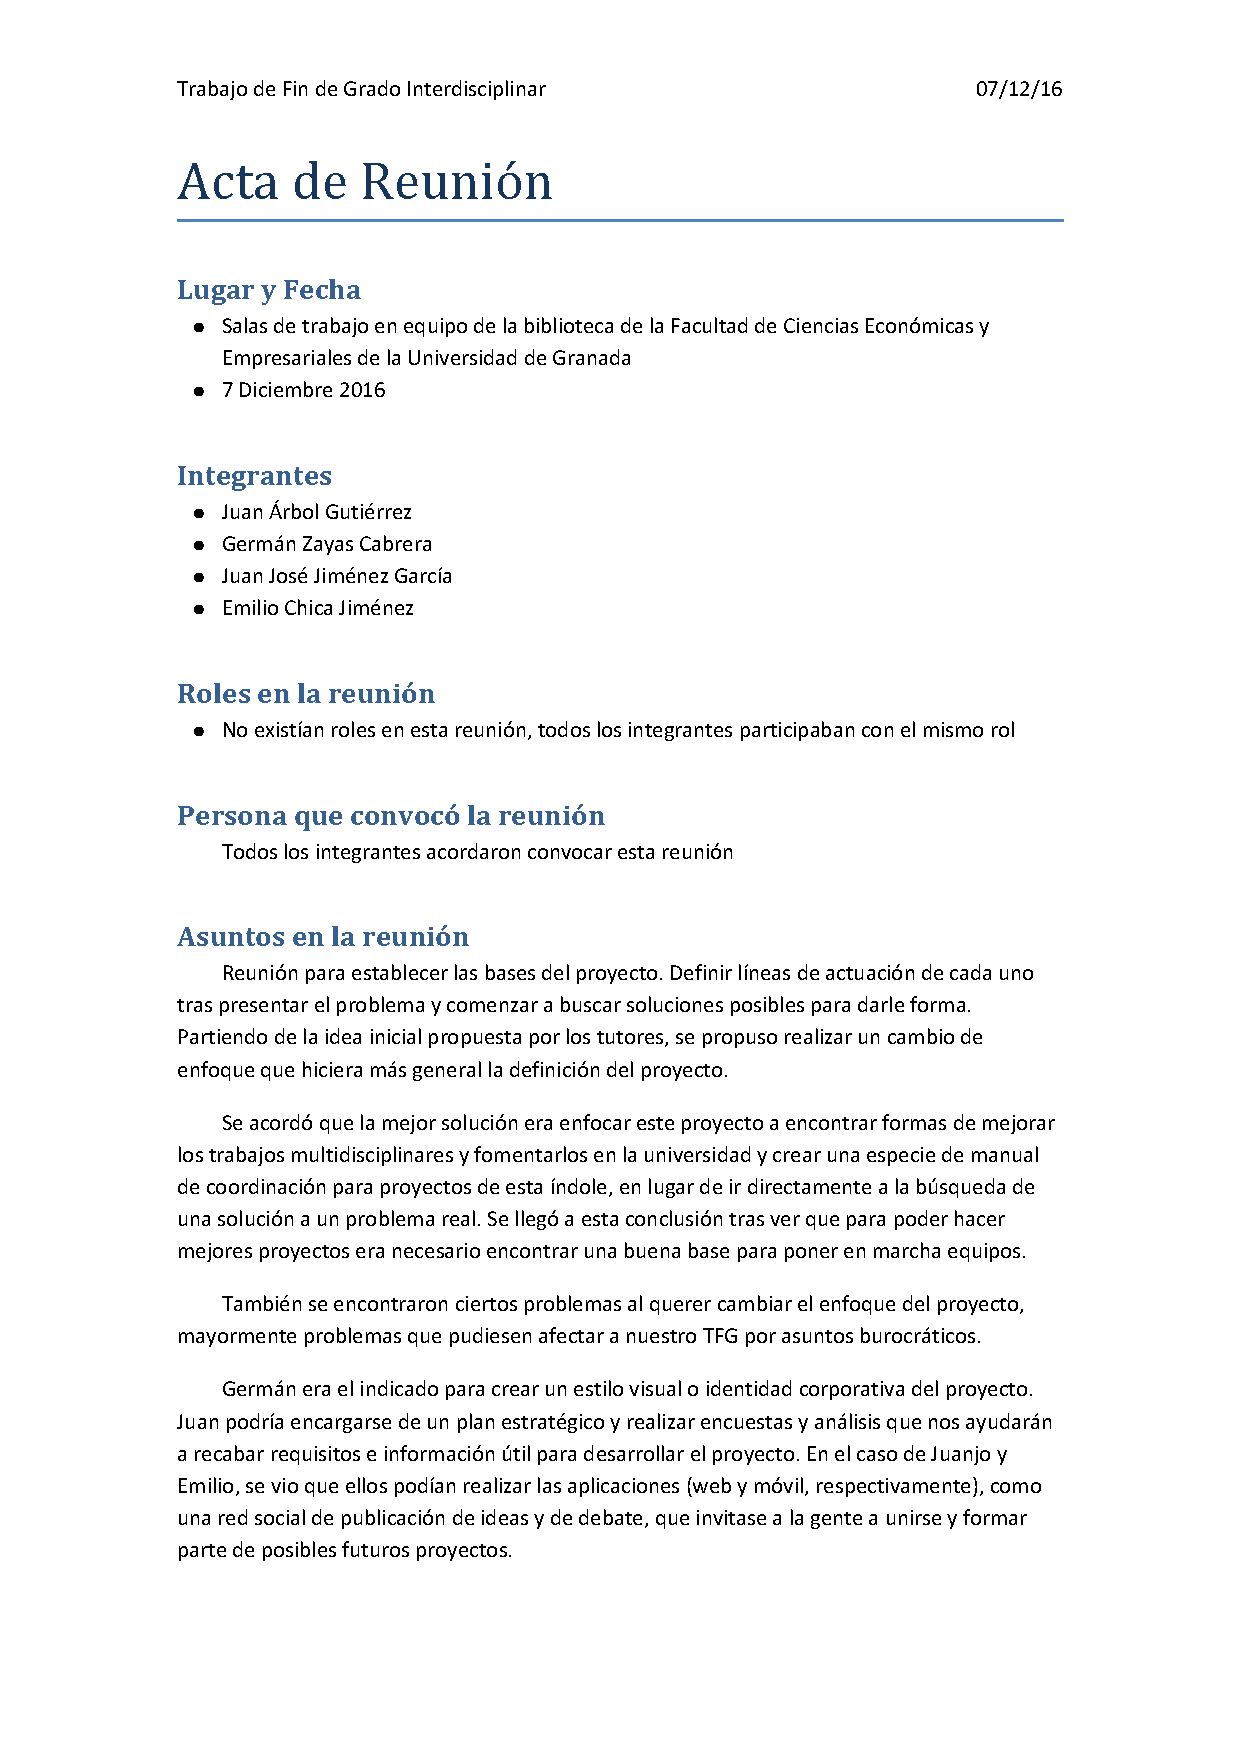
\includepdf[pages=1-]{meetings/02.pdf}
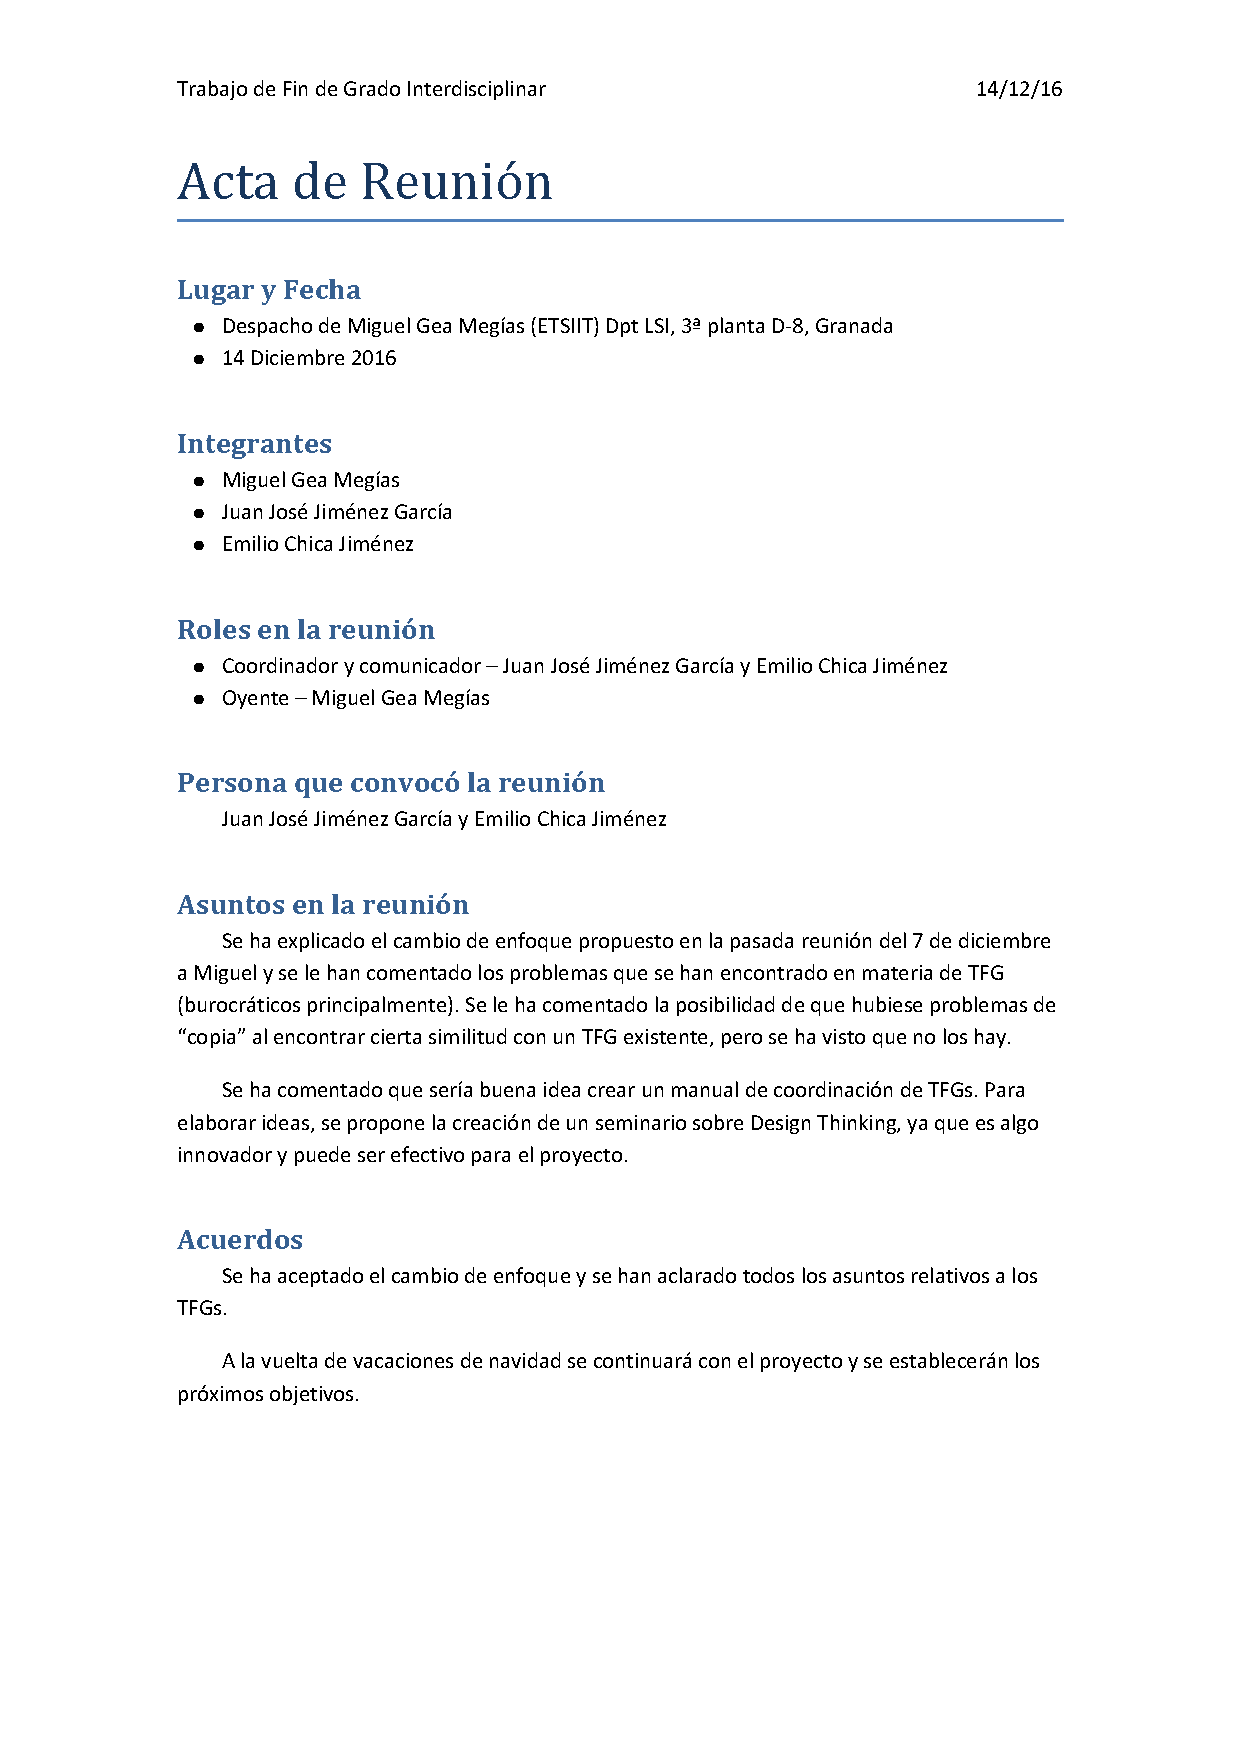
\includepdf[pages=1-]{meetings/03.pdf}
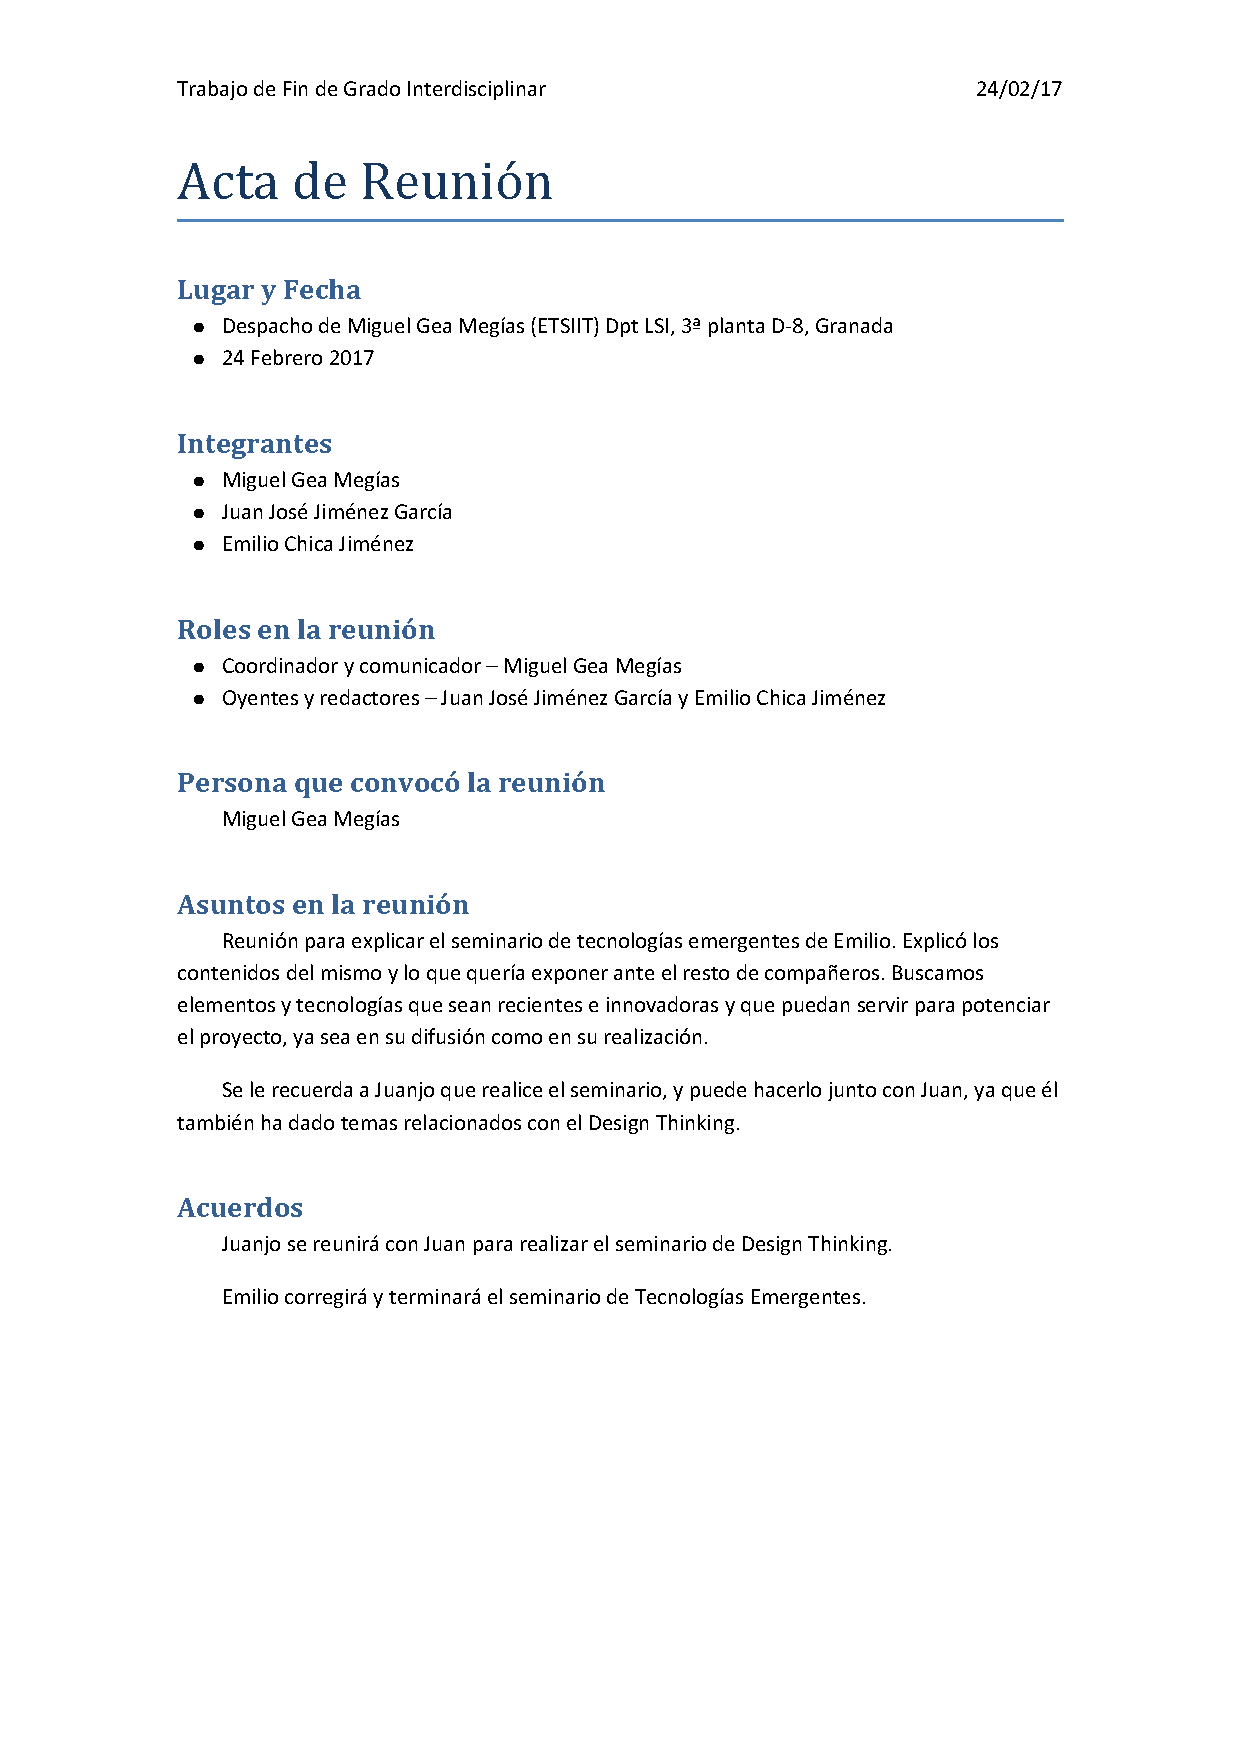
\includepdf[pages=1-]{meetings/04.pdf}
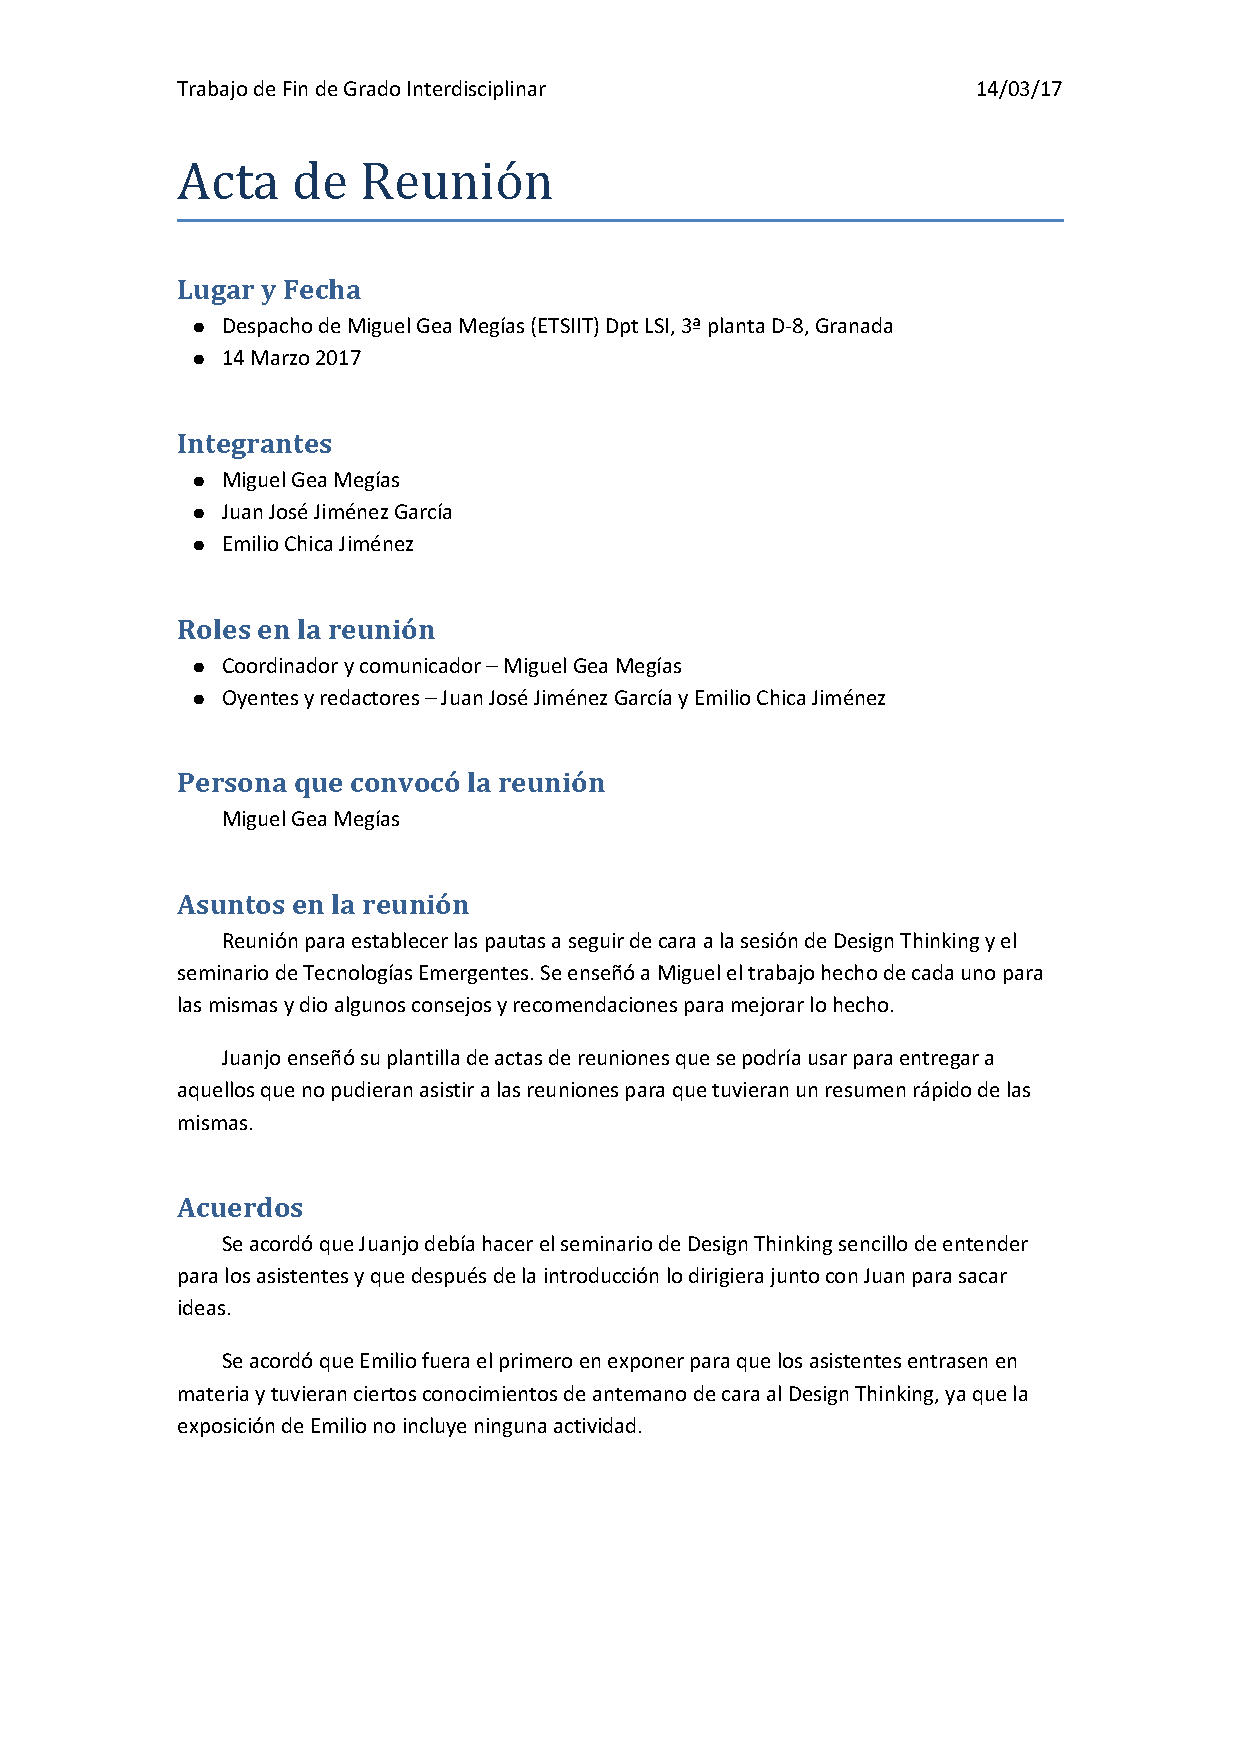
\includepdf[pages=1-]{meetings/05.pdf}
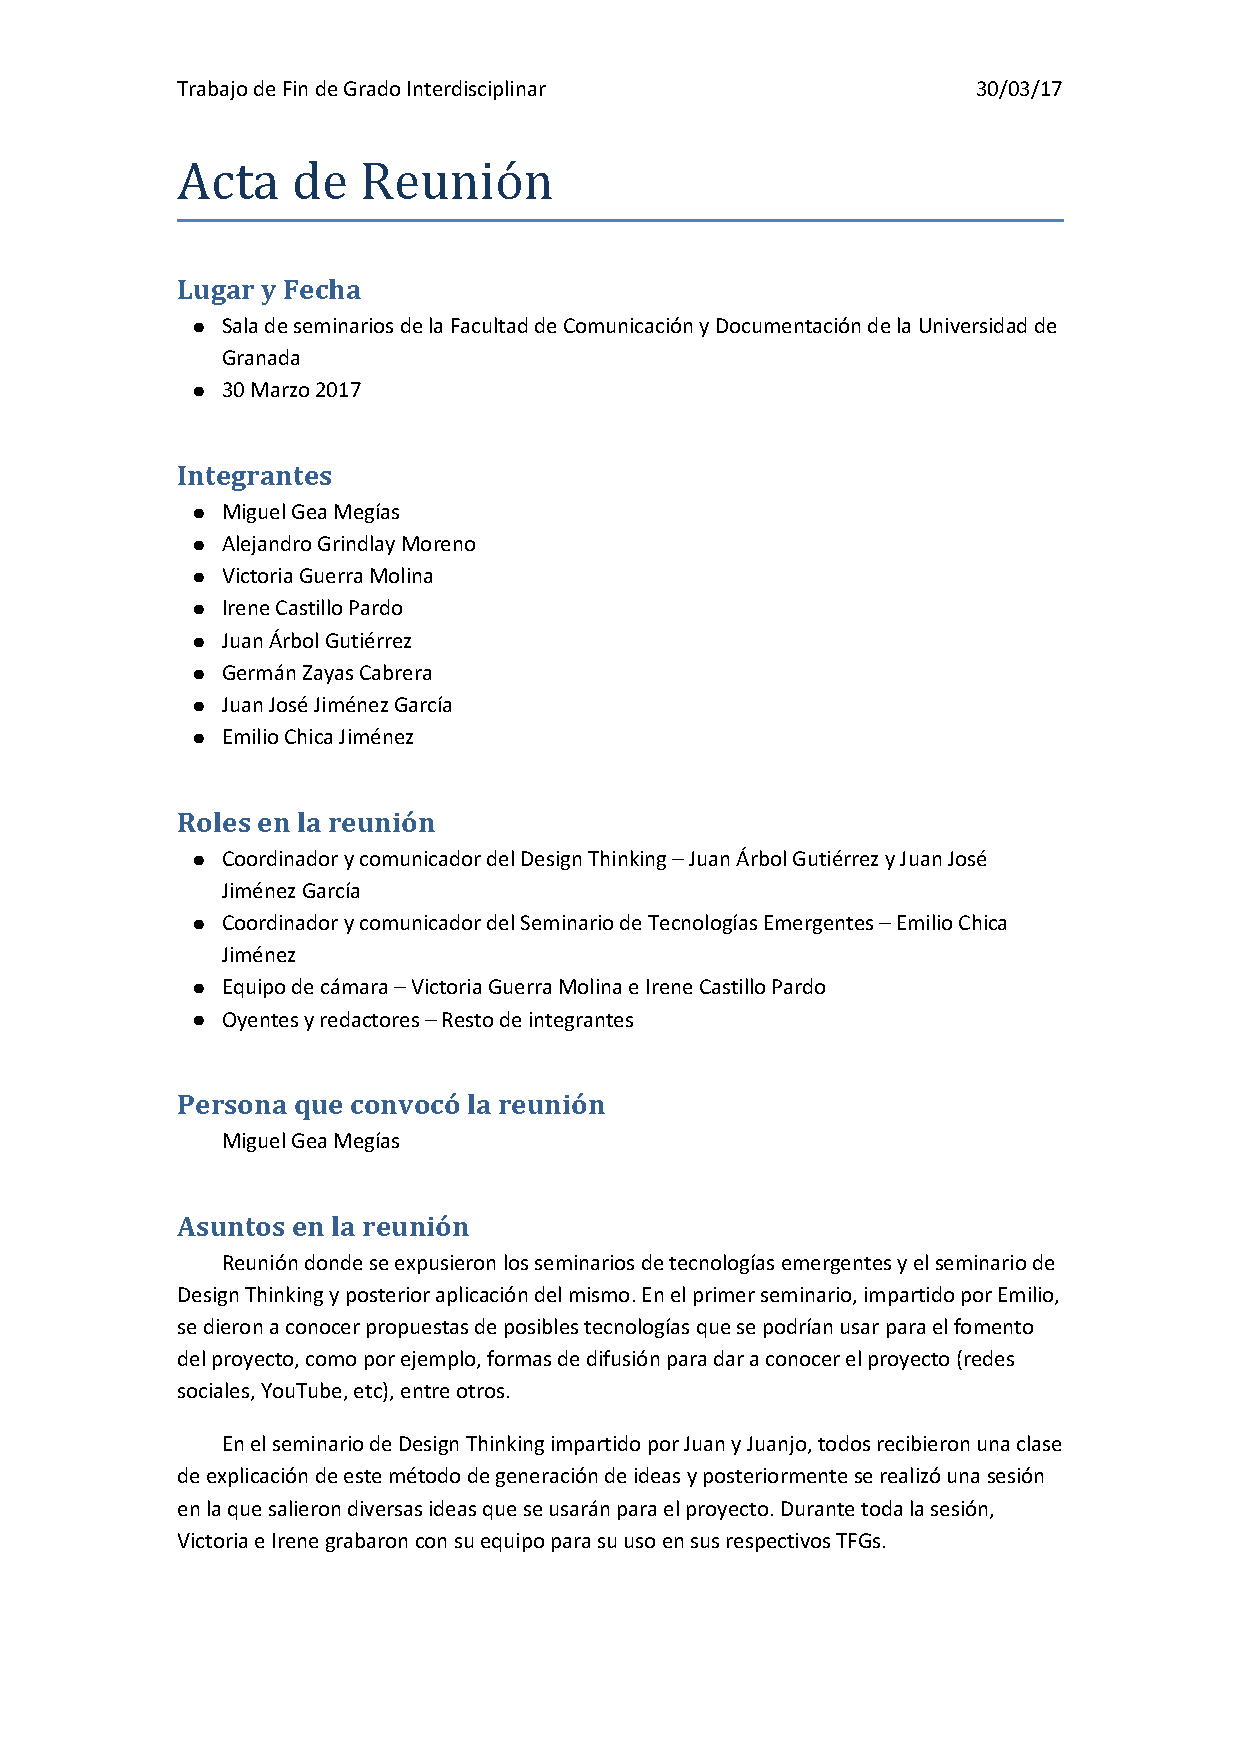
\includepdf[pages=1-]{meetings/06.pdf}
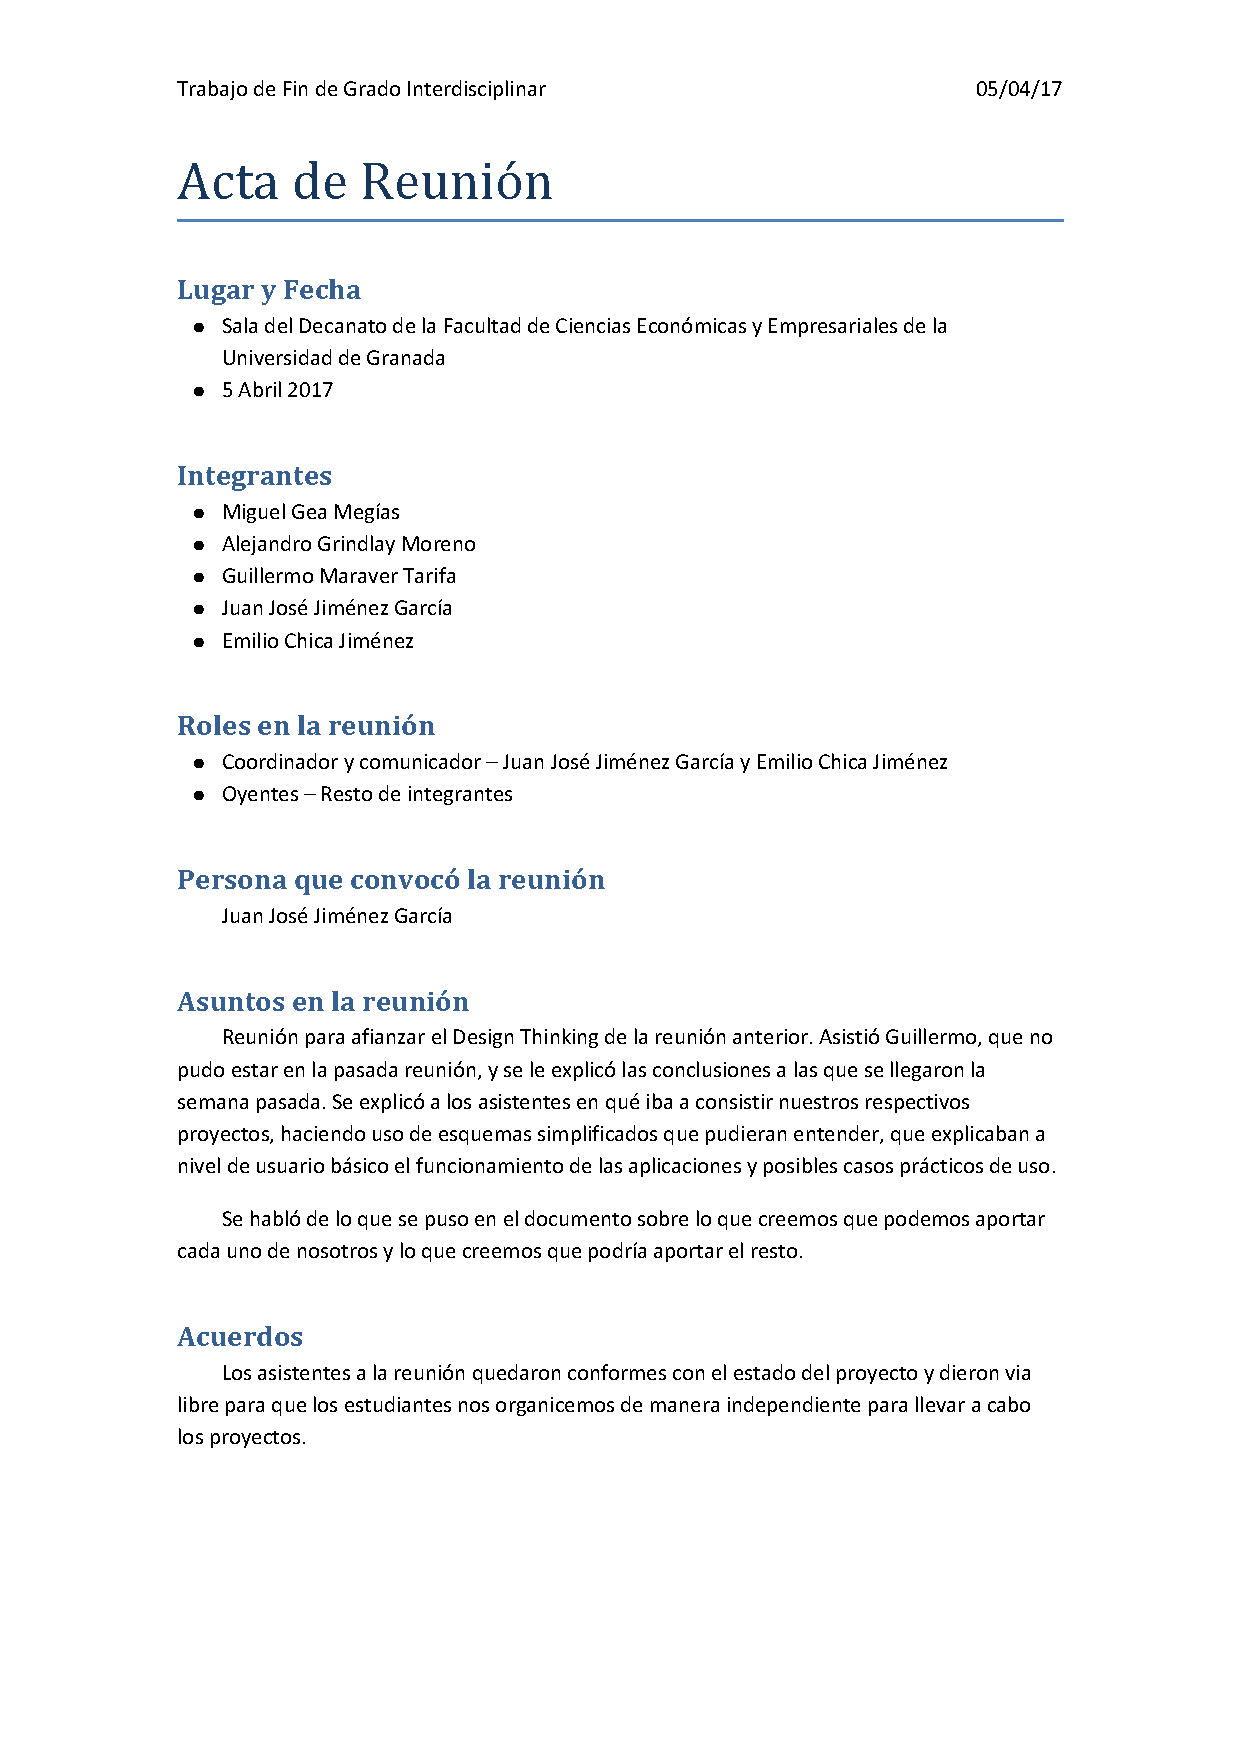
\includepdf[pages=1-]{meetings/07.pdf}
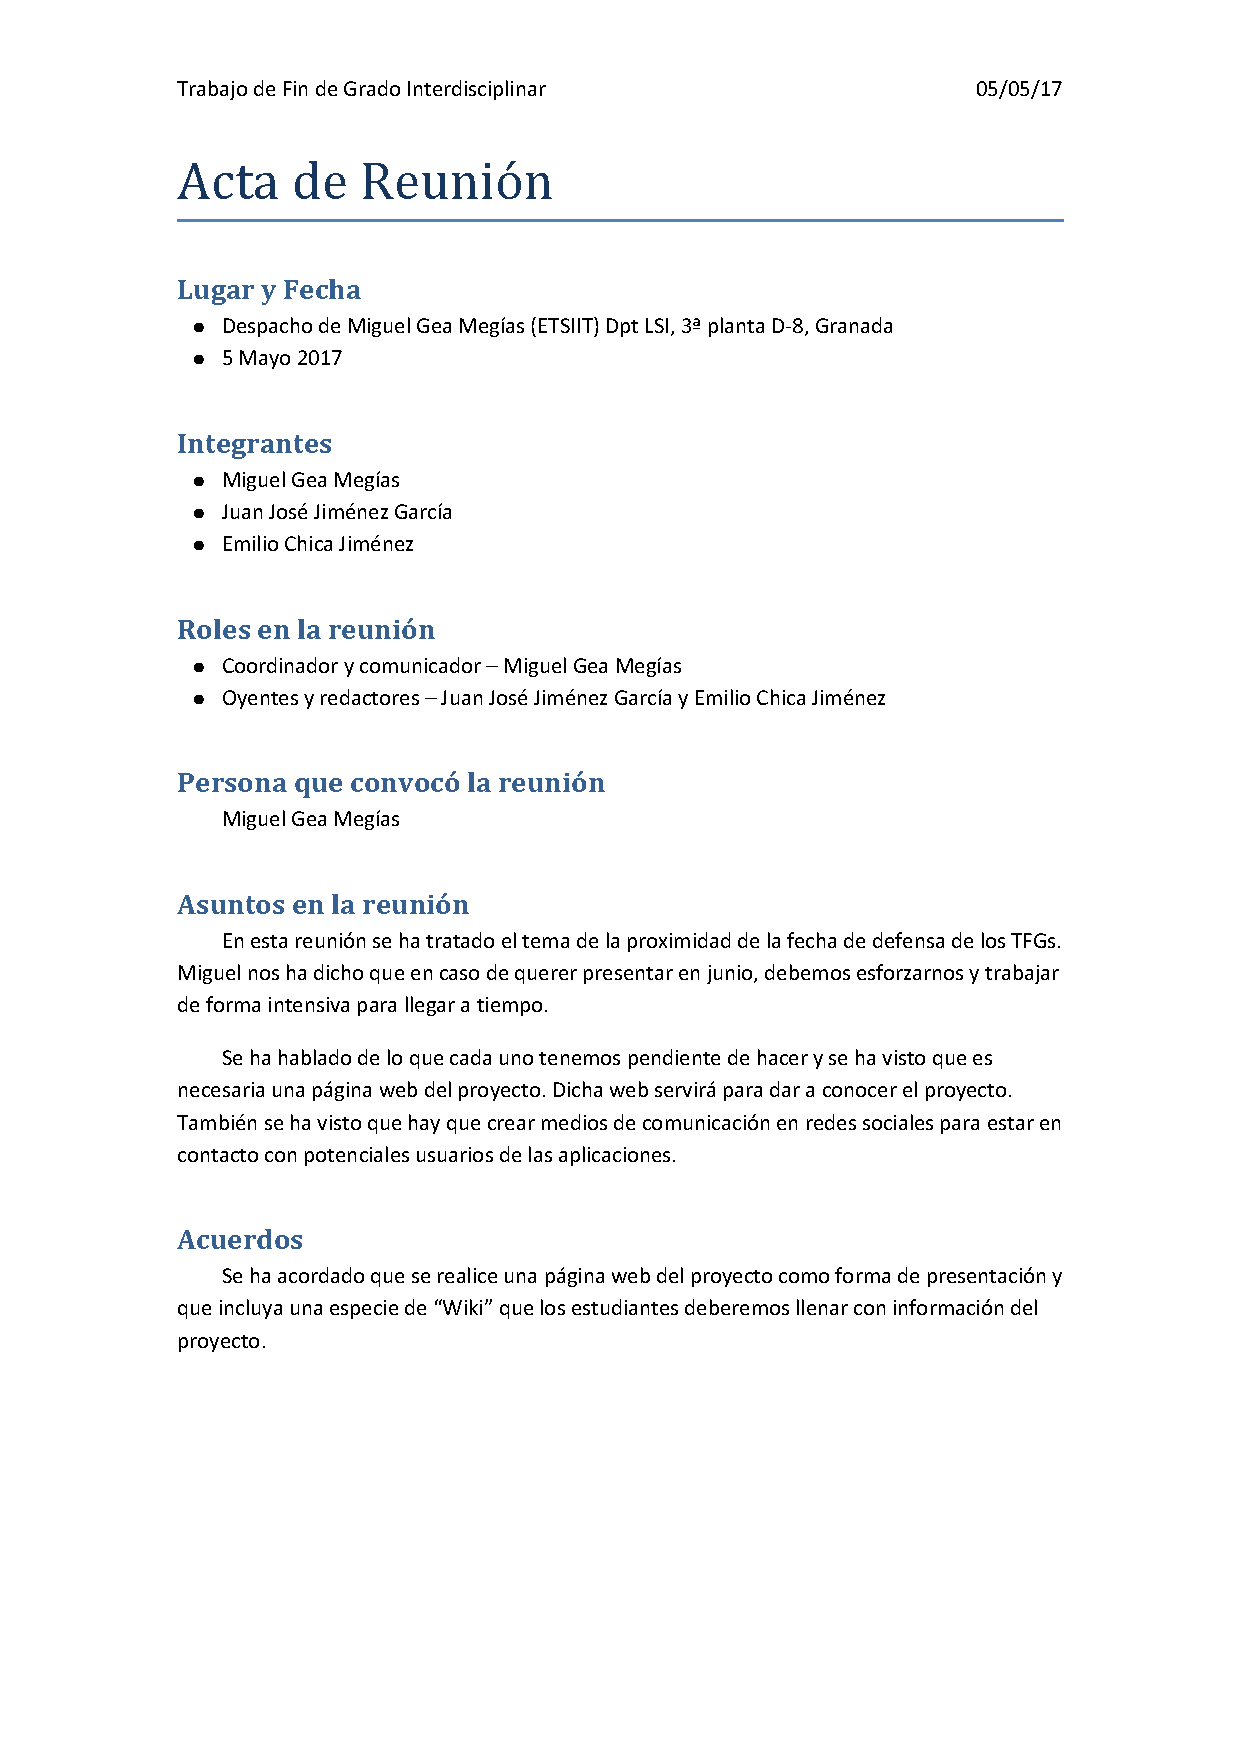
\includepdf[pages=1-]{meetings/08.pdf}
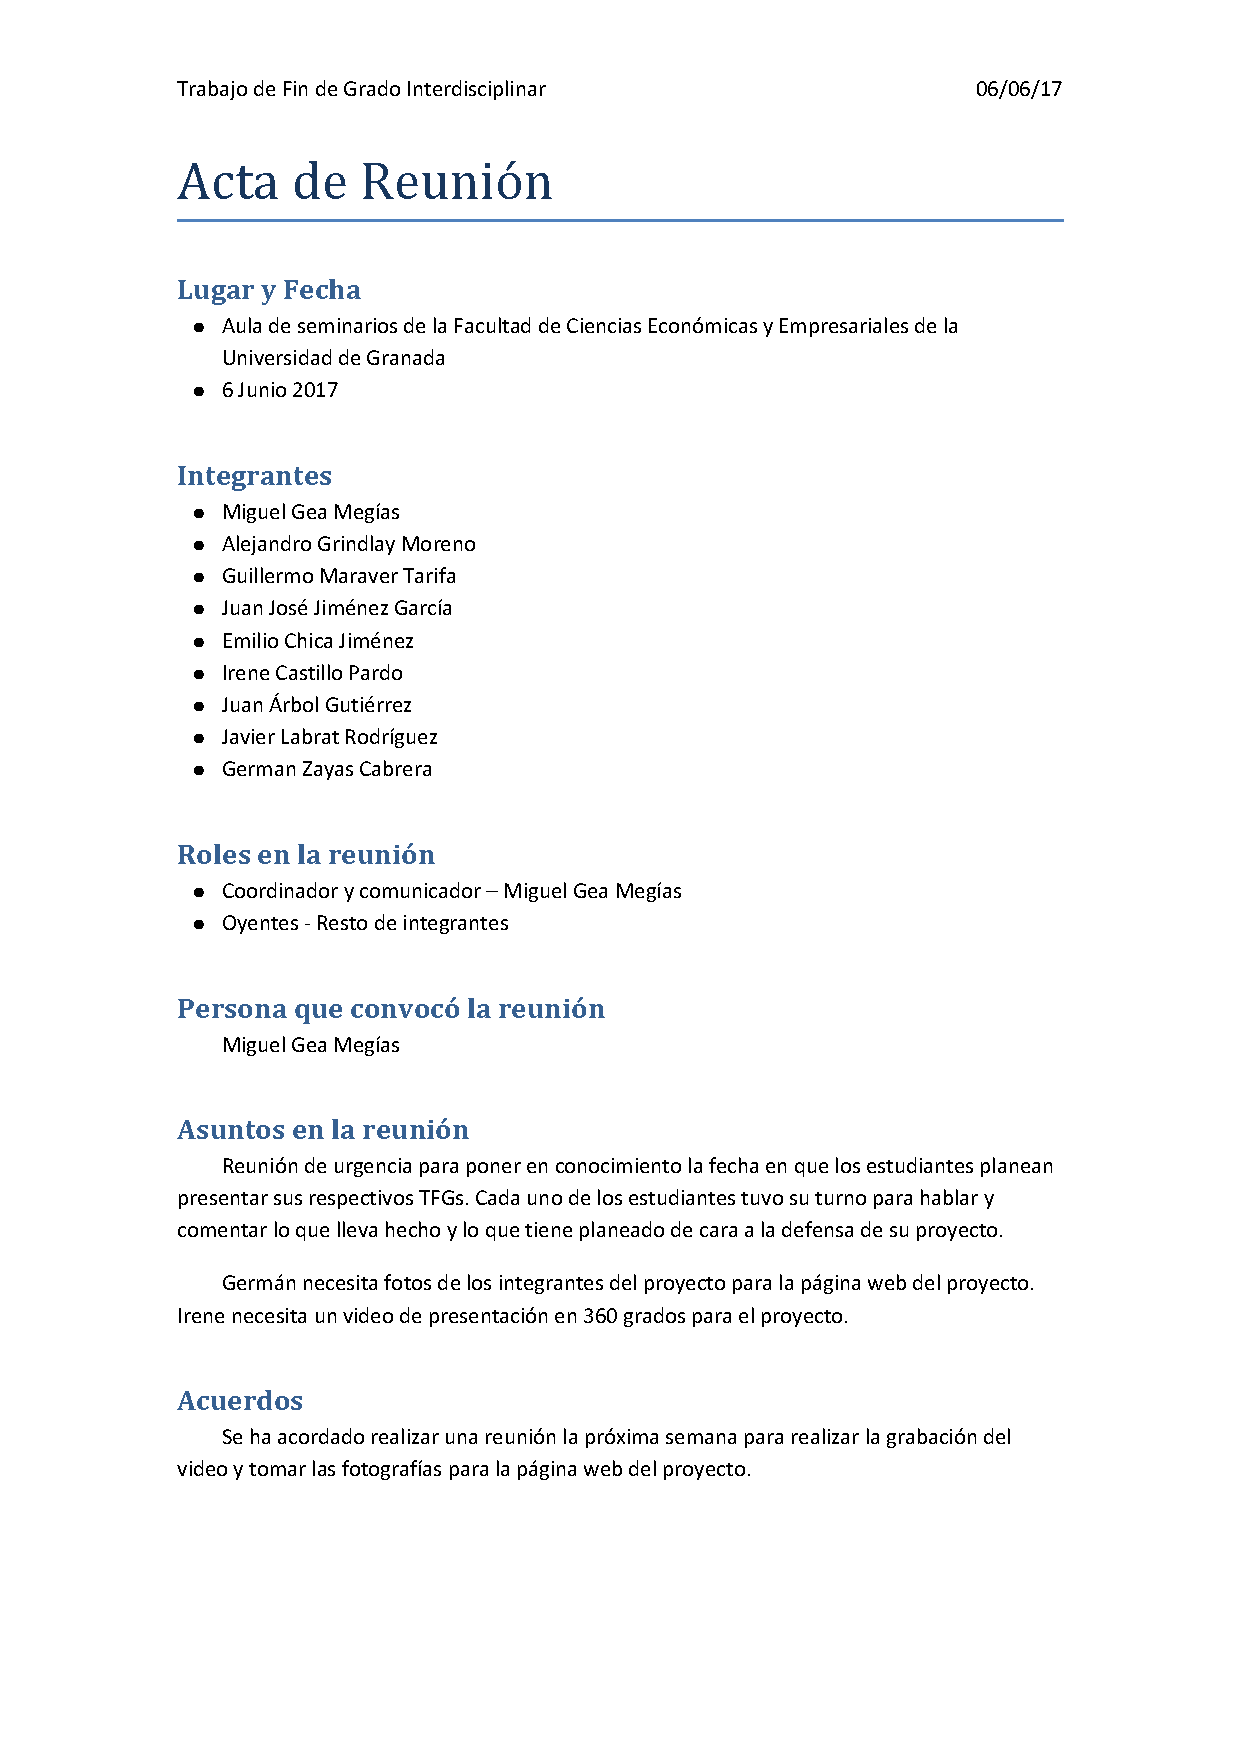
\includepdf[pages=1-]{meetings/09.pdf}
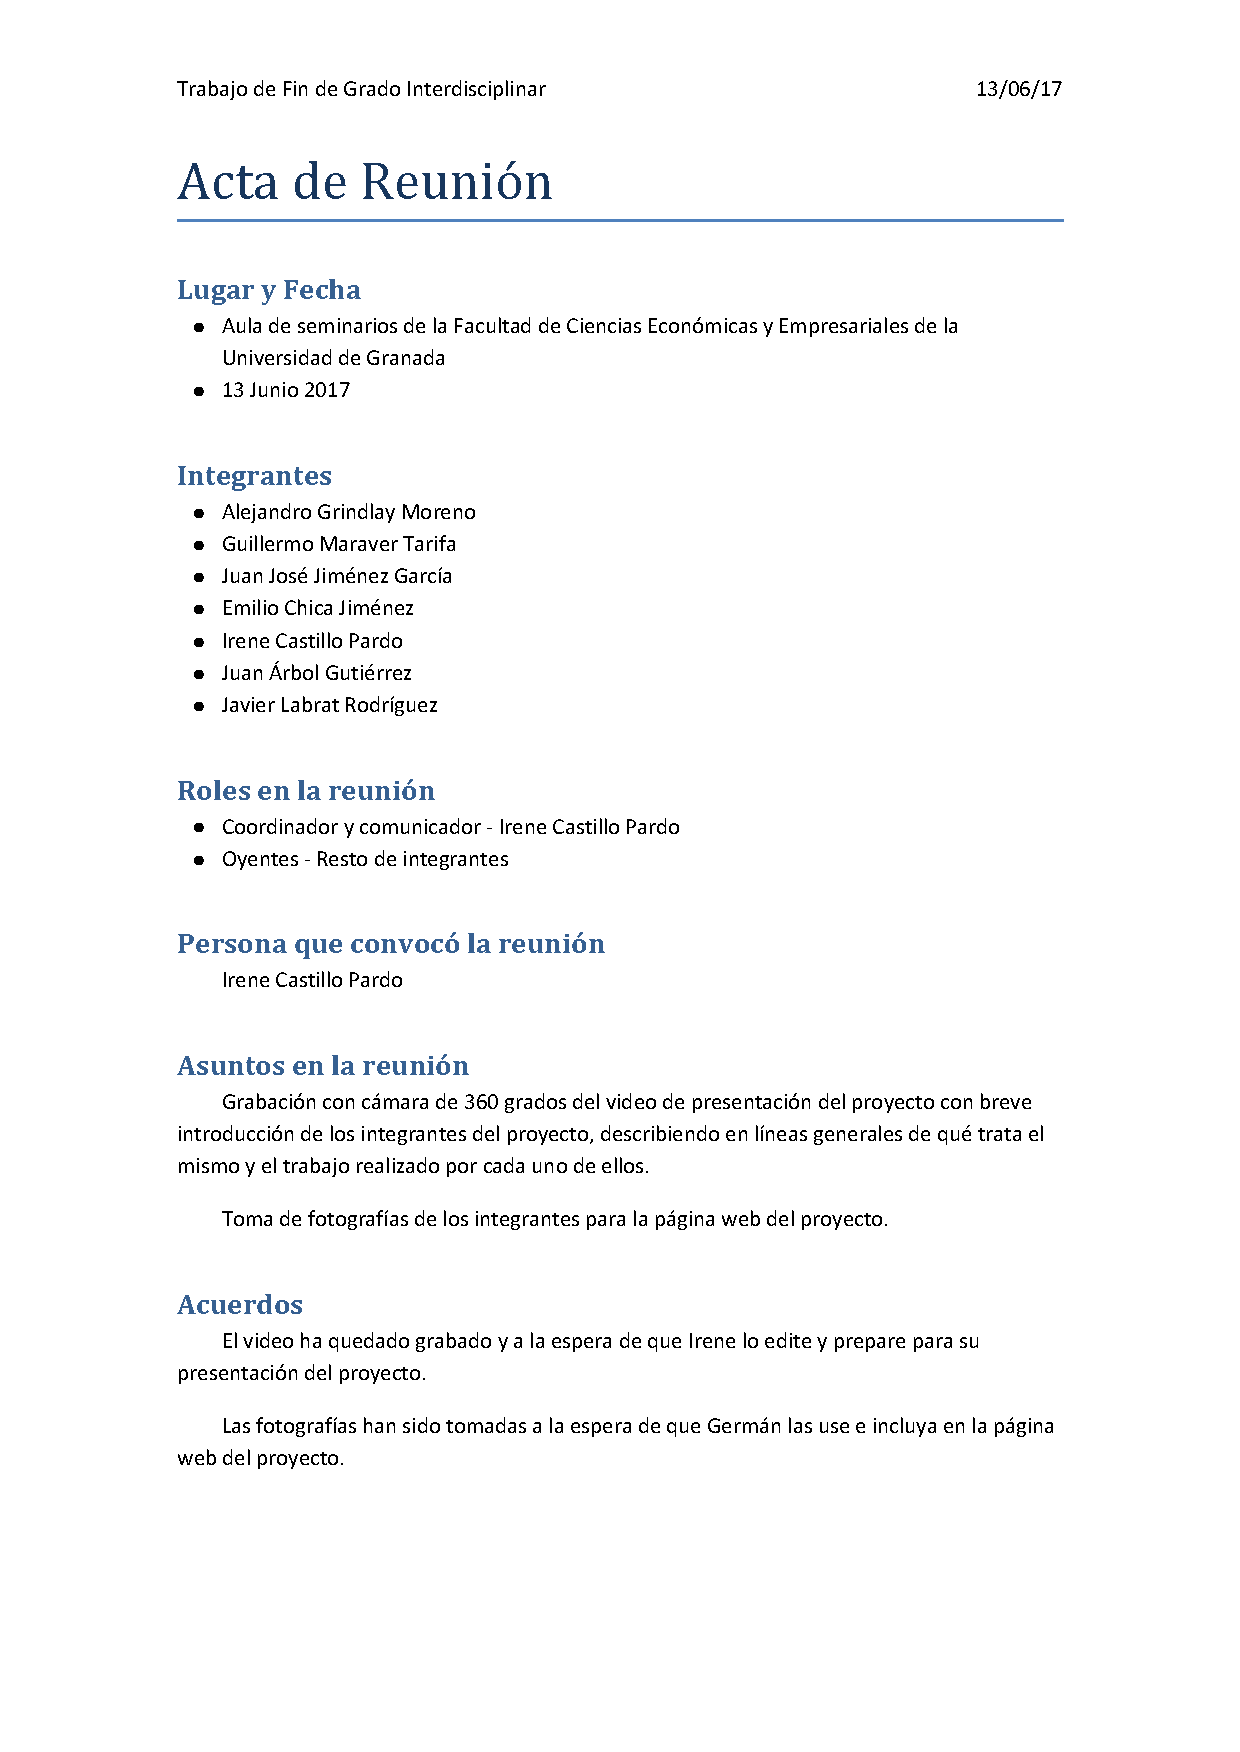
\includepdf[pages=1-]{meetings/10.pdf}


\backmatter
\begingroup
	\setlength\parindent{0pt}
	\chapter{Glosario de términos}

\begin{description}
    \item[Equipo multidisciplinar] Conjunto de personas, con diferentes formaciones académicas y experiencias profesionales, que operan en conjunto, durante un tiempo determinado, abocados a resolver un problema complejo, es decir, que tienen un objetivo común. Cada individuo es consciente de su papel y del papel de los demás, y trabajan en conjunto bajo la dirección de un coordinador.
    \item[StartUp] Empresa emergente que busca arrancar, emprender o montar un negocio, generalmente apoyada en la tecnología para su desarrollo. Son ideas que innovan el mercado y buscan facilitar los procesos complicados, enfocadas a diferentes temas y usos. Generalmente son empresas asociadas a la innovación, al desarrollo de tecnologías, al diseño web o al desarrollo web.
    \item[Sinergia] La sinergia es una propiedad inherente de los sistemas que establece que las interacciones entre las partes o componentes de un sistema generan un valor agregado mayor al que se lograría si cada componente funcionara por separado.\\
    Aplicado al trabajo en equipo, surgen sinergias cuando la colaboración entre miembros produce más resultados que haciéndo cada uno su parte sin contar con el otro.
    \item[Framework de desarrollo] Es una estructura conceptual y tecnológica de asistencia definida, normalmente, con artefactos o módulos concretos de software, que puede servir de base para la organización y desarrollo de software. Típicamente, puede incluir soporte de programas, bibliotecas, y un lenguaje interpretado, entre otras herramientas, para así ayudar a desarrollar y unir los diferentes componentes de un proyecto.
    \item[Diseño adaptable] El diseño adaptable establece que un sistema informático debe ser reactivo a la interacción del usuario con el mismo y al entorno en el que se encuentra. Esto quiere decir que ha de ``adaptarse'' a todo tipo de dispositivos donde se esté ejecutando o visualizando.
    \item[Diseño \textit{Mobile First}] es una filosofía de diseño que establece que todo desarrollo debe centrar su diseño en visualizar cómo se vería en un dispositivo móvil, y a partir de ese punto ampliar el tamaño de la pantalla e ir reorganizando los elementos.\\
    Por lo general, el diseño \textit{mobile first} comienza apilando uno encima de otro los elementos de la interfaz, y a medida que se gana espacio horizontal, colocar en este los elementos que estaban al fondo.
\end{description}

\endgroup

\newpage
\begin{thebibliography}{99}
	\addcontentsline{toc}{chapter}{Bibliografía}

\bibitem{globalizacion} {\tt Globalización - Wikipedia}\\
\url{https://es.wikipedia.org/wiki/Globalizaci%C3%B3n}

\bibitem{ugremprende} {\tt UGR Emprendedora - Página principal}\\
\url{https://ugremprendedora.ugr.es/}

\bibitem{h2020} {\tt Horizon 2020 - Página principal}\\
\url{https://ec.europa.eu/programmes/horizon2020/}

\bibitem{agilereport} {\tt Top 10 Insights from the 11th Annual State of Agile Report}\\
\url{https://explore.versionone.com/state-of-agile/top-10-insights-from-the-11th-annual-state-of-agile-report-2}

\bibitem{health1} {\tt PubMed Central - Multidisciplinary in-hospital teams improve patient outcomes: A review}\\
\url{https://www.ncbi.nlm.nih.gov/pmc/articles/PMC4173201/}

\bibitem{health2} {\tt PubMed Central - Benefits of multidisciplinary teamwork in the management of breast cancer}\\
\url{https://www.ncbi.nlm.nih.gov/pmc/articles/PMC3929250/}

\bibitem{neuroped} {\tt Imagen original de NeuroPed - Enlace}\\
\url{http://www.neuroped.es/equipo-multidisciplinar/}

\bibitem{medialabugr} {\tt Medialab UGR - Página principal}\\
\url{http://medialab.ugr.es/}

\bibitem{linkuma} {\tt Link by UMA-ATech (Universidad de Málaga) - Página principal}\\
\url{http://www.link.uma.es/}

\bibitem{linkedin} {\tt LinkedIn - Página principal}\\
\url{https://es.linkedin.com/}

\bibitem{kickstarter} {\tt Kickstarter - Página principal}\\
\url{https://www.kickstarter.com/}

\bibitem{contentwater} {\tt Imagen original de Wikimedia - Enlace}\\
\url{https://commons.wikimedia.org/wiki/File:Content_is_like_water.png}

\bibitem{bootstrap} {\tt Bootstrap Framework - Página principal}\\
\url{https://getbootstrap.com/}

\bibitem{framework} {\tt Framework - Wikipedia}\\
\url{https://es.wikipedia.org/wiki/Framework}

\bibitem{startup} {\tt Startup - Wikipedia}\\
\url{https://es.wikipedia.org/wiki/Empresa_emergente}

\bibitem{whatsapp} {\tt WhatsApp - Página oficial}\\
\url{https://www.whatsapp.com/}

\bibitem{slack} {\tt Slack - Página oficial}\\
\url{https://slack.com/}

\bibitem{googlecalendar} {\tt Google Calendar - Página oficial}\\
\url{https://www.google.com/calendar}

\bibitem{googledrive} {\tt Google Drive - Página oficial}\\
\url{https://www.google.com/drive}

\bibitem{laravel} {\tt Laravel - Documentación oficial}\\
\url{https://laravel.com/docs/5.5}

\bibitem{xampp} {\tt XAMPP - Página oficial}\\
\url{https://www.apachefriends.org/es/index.html}





















% \subsubsection*{Libros consultados durante la realización del proyecto:}
% \bibitem{stevekrug}
% Steve Krug.
% \newblock {\em Don't make me think! : a common sense approach to web usability.}
% \newblock New Riders, 2006.
% \newblock ISBN: 0321344758.
%
% \bibitem{jakonielsen}
% Jakob Nielsen.
% \newblock {\em 10 Usability Heuristics for User Interface Design.}
% \newblock Nielsen Norman Group, 1995.
%
% \bibitem{melenaalva}
% María Elena Alva Obeso.
% \newblock {\em Metodología de medición y evaluación de la usabilidad en sitios Web educativos.}
% \newblock Universidad de Oviedo, 2005.
% \newblock ISBN: 9788483175842.
%
% \bibitem{ericreiss}
% Eric Reiss.
% \newblock {\em Usable usability: simple steps for making stuff better .}
% \newblock John Wiley \& Sons, Inc., 2012.
% \newblock ISBN: 9781118185476.
%
% \subsubsection*{Artículos sobre las metodologías utilizadas en el proyecto:}
% \bibitem{art_14} `'The Distributed Course'. Stephen Downes. 2008. \url{https://sites.google.com/site/themoocguide/3-cck08---the-distributed-course}
%
% \bibitem{art_13} ``Top Universities Test the Online Appeal of Free''. Richard Pérez-Peña. 18/07/2012. \url{http://www.nytimes.com/2012/07/18/education/top-universities-test-the-online-appeal-of-free.html}
%
% \bibitem{art_12} `'Cuando un profesor de la Gran Depresión predijo la educación online'. Jonathan Préstamo. 09/06/2017. \url{http://www.teknoplof.com/2017/06/09/cuando-profesor-la-gran-depresion-predijo-la-educacion-online/}
%
% \bibitem{art_11} ``Legislación sobre accesibilidad web en España, Europa y otros países''. Olga Carreras Montoto. 11/12/2016. \url{https://olgacarreras.blogspot.com.es/2005/01/referencia-sobre-legislacin-espaola.html}
%
% \bibitem{art_11} ``Having problems with SSL by René Breedveld''. René Breedveld. 30/10/2015. \url{https://github.com/dmuneras/moodle-theme_archaius/wiki/Having-problems-with-SSL-byRen\%C3\%A9-Breedveld}
%
% \bibitem{art_10} ``An user can enter with an admin role only copying valid sessionID from another computer with the same IP address.''. Juan Carlos Molina Giménez, 18/01/2016. \url{https://tracker.moodle.org/browse/MDL-52812}
%
% \bibitem{art_09} ``mdl\_log now a legacy table''. Stuart Mealor, 30/05/2014. \url{http://elearningblog.moodlebites.com/mod/oublog/viewpost.php?post=90}
%
% \bibitem{art_08} ``ARP spoofing''. Wikipedia, última edición: 01/05/2017 \url{https://en.wikipedia.org/wiki/ARP_spoofing}
%
% \bibitem{art_07} ``ARP and ICMP redirection games''. Yuri Volobuev, 19/11/1997. \url{http://insecure.org/sploits/arp.games.html}
%
% \bibitem{art_06} ``Presto Parking: ¿Un sitio web PCI-Compliant sin HTTPs?''. José C. A., 17/04/2017. \url{http://www.elladodelmal.com/2017/04/presto-parking-un-sitio-web-pci.html}
%
% \bibitem{art_05} ``Corregidas cuatro vulnerabilidades en Moodle''. Antonio Ropero, 3/04/2017. \url{http://unaaldia.hispasec.com/2017/04/corregidas-cuatro-vulnerabilidades-en.html}
%
% \bibitem{art_04} ``Múltiples vulnerabilidades en Moodle''. Antonio Ropero, 25/11/2016. \url{http://unaaldia.hispasec.com/2016/11/multiples-vulnerabilidades-en-moodle.html}
%
% \bibitem{art_03} ``Important Announcement Regarding YUI''. Julien Lecomte, 29/08/2014. \url{https://yahooeng.tumblr.com/post/96098168666/important-announcement-regarding-yui}
%
% \bibitem{art_02} ``Learning logs: How long are your users online? Analytics Part 2''. James Ballard, 01/06/2015. \url{https://infiniterooms.wordpress.com/2015/06/01/learning-logs/}
%
% \bibitem{art_01} ``Reckon you've seen some stupid security things? Here, hold my beer...''. Troy Hunt, 28/04/2017. \url{https://www.troyhunt.com/reckon-youve-seen-some-stupid-security-things-here-hold-my-beer/}
%
% \bigskip
% \subsubsection*{Páginas de consulta sobre licencias, desarrollo y uso del software analizado}
% \bibitem{CC} {\tt Creative Commons Share Alike 4.0}. \url{https://creativecommons.org/licenses/by-sa/4.0/}
% \bibitem{moodle} {\tt moodle}. \url{https://docs.moodle.org}
% \bibitem{wikibooks} Wikibooks ({\tt LaTeX}). \url{https://en.wikibooks.org/wiki/LaTeX}
% \bibitem{ettercap} {\tt ettercap}. \url{https://github.com/Ettercap/ettercap}
% \bibitem{statuscake} {\tt StatusCake}. \url{https://statuscake.com/kb}
% \bibitem{urlscan} {\tt urlscan.io}. \url{https://urlscan.io/about/}
% \bibitem{moodleplugin} {\tt material download moodle plugin}. \url{https://github.com/TUM-MZ/moodle-block_material-download}
% \bibitem{moodletheme} {\tt archaius theme}. \url{https://moodle.org/plugins/theme_archaius}
% \bibitem{rae} {\tt Diccionario RAE}. \url{http://dle.rae.es/}
% \bibitem{w3c} {\tt W3C}. \url{https://www.w3.org/}
% \bibitem{wcag} {\tt WCAG}. \url{https://www.w3.org/TR/WCAG/}
% \bibitem{taw} {\tt T.A.W.}. \url{http://www.tawdis.net/}
% \bibitem{tenon} {\tt tenon.io}. \url{https://tenon.io}
% \bibitem{codesniffer} {\tt HTML CodeSniffer}. \url{http://squizlabs.github.io/HTML_CodeSniffer/}
% \bibitem{openwrt} {\tt OpenWRT}. \url{https://wiki.openwrt.org/toh/huawei/hg556a}
% \bibitem{moodledb} Moodle Database Schema. \url{https://docs.moodle.org/dev/Database_Schema}
% \bibitem{mooc} MOOC. \url{https://es.wikipedia.org/wiki/Massive_Open_Online_Course}
%
% \bigskip
% \subsubsection*{Otro material}
% \begin{itemize}
% 	\item Diversas consultas puntuales al sitio {\tt Stack OverFlow}.
% 	\item Material docente de las asignaturas \textbf{Fundamentos de Ingeniería del Software}, \textbf{Seguridad en Sistemas Operativos}, \textbf{Desarrollo de Aplicaciones para Internet}, \textbf{Diseño y Desarrollo de Sistemas de Información}, \textbf{Seguridad en Sistemas Operativos} y \textbf{Sistemas de Información Basados en Web} impartidas en \textbf{Grado en Ingeniería Informática} en la \textbf{Universidad de Granada}.
% \end{itemize}

\end{thebibliography}

\newpage
\thispagestyle{empty}

\end{document}
